% SI tables portion (ST1–ST10 + paired SF1–SF9 figure blocks in the fragments).
% Compile from this directory:
%   latexmk -pdf -interaction=nonstopmode main.tex
%
% Generated fragments live in ../../figures/ST*.tex (produced by the SI wrapper).
\documentclass[11pt]{article}
% Shared packages for SI table/figure masters (input by each master).
\usepackage[margin=0.6in]{geometry}
\usepackage{booktabs}
\usepackage{longtable}
\usepackage{caption}
\usepackage{hyperref}
\usepackage{graphicx}
\usepackage{float}
\usepackage{amsmath}
\usepackage{enumitem}
\graphicspath{{../../figures/}{../}{./}}
\setlength{\parindent}{0pt}
\pagestyle{plain}


\begin{document}

% ST1 — all receptors
% In your document preamble: \usepackage{booktabs}, \usepackage{hyperref}, \usepackage{longtable}, \usepackage{caption}
\scriptsize
\setlength{\tabcolsep}{3pt}
\begin{longtable}{llllrr@{\hspace{0.8cm}}llllrr}
\captionsetup{labelformat=empty}
\caption{\textbf{SI Table S1. Data for all receptors in this study}}
\label{tab:st1} \\
\toprule
apo\_pdb & holo\_pdb & apo\_bmrb & holo\_bmrb & F1 & MCC & apo\_pdb & holo\_pdb & apo\_bmrb & holo\_bmrb & F1 & MCC \\
\midrule
\endfirsthead
\caption[]{(continued)} \\
\toprule
apo\_pdb & holo\_pdb & apo\_bmrb & holo\_bmrb & F1 & MCC & apo\_pdb & holo\_pdb & apo\_bmrb & holo\_bmrb & F1 & MCC \\
\midrule
\endhead
\bottomrule
\endfoot
\bottomrule
\endlastfoot
 & \href{https://www.rcsb.org/structure/1YWI}{1YWI} & \href{https://bmrb.io/data_library/summary/index.php?bmrbId=6658}{6658} & \href{https://bmrb.io/data_library/summary/index.php?bmrbId=6659}{6659} & 0.78 & 0.72 & \href{https://www.rcsb.org/structure/1SSF}{1SSF} & \href{https://www.rcsb.org/structure/2LVM}{2LVM} & \href{https://bmrb.io/data_library/summary/index.php?bmrbId=5878}{5878} & \href{https://bmrb.io/data_library/summary/index.php?bmrbId=18579}{18579} & 0.31 & 0.20 \\
 & \href{https://www.rcsb.org/structure/2FIN}{2FIN} & \href{https://bmrb.io/data_library/summary/index.php?bmrbId=5073}{5073} & \href{https://bmrb.io/data_library/summary/index.php?bmrbId=7024}{7024} & 0.65 & 0.52 &  & \href{https://www.rcsb.org/structure/2M56}{2M56} & \href{https://bmrb.io/data_library/summary/index.php?bmrbId=17415}{17415} & \href{https://bmrb.io/data_library/summary/index.php?bmrbId=19038}{19038} & 0.12 & 0.18 \\
 & \href{https://www.rcsb.org/structure/2ROZ}{2ROZ} & \href{https://bmrb.io/data_library/summary/index.php?bmrbId=10235}{10235} & \href{https://bmrb.io/data_library/summary/index.php?bmrbId=10236}{10236} & 0.59 & 0.50 &  & \href{https://www.rcsb.org/structure/2B0F}{2B0F} & \href{https://bmrb.io/data_library/summary/index.php?bmrbId=5659}{5659} & \href{https://bmrb.io/data_library/summary/index.php?bmrbId=6823}{6823} & 0.27 & 0.18 \\
 & \href{https://www.rcsb.org/structure/5I22}{5I22} & \href{https://bmrb.io/data_library/summary/index.php?bmrbId=4871}{4871} & \href{https://bmrb.io/data_library/summary/index.php?bmrbId=30010}{30010} & 0.55 & 0.49 &  & \href{https://www.rcsb.org/structure/2YS5}{2YS5} & \href{https://bmrb.io/data_library/summary/index.php?bmrbId=11095}{11095} & \href{https://bmrb.io/data_library/summary/index.php?bmrbId=11094}{11094} & 0.35 & 0.18 \\
 & \href{https://www.rcsb.org/structure/2LBM}{2LBM} & \href{https://bmrb.io/data_library/summary/index.php?bmrbId=15001}{15001} & \href{https://bmrb.io/data_library/summary/index.php?bmrbId=17569}{17569} & 0.60 & 0.46 & \href{https://www.rcsb.org/structure/6VED}{6VED} & \href{https://www.rcsb.org/structure/2L3R}{2L3R} & \href{https://bmrb.io/data_library/summary/index.php?bmrbId=30703}{30703} & \href{https://bmrb.io/data_library/summary/index.php?bmrbId=17200}{17200} & 0.30 & 0.18 \\
\href{https://www.rcsb.org/structure/7JMY}{7JMY} & \href{https://www.rcsb.org/structure/7JYN}{7JYN} & \href{https://bmrb.io/data_library/summary/index.php?bmrbId=30782}{30782} & \href{https://bmrb.io/data_library/summary/index.php?bmrbId=30790}{30790} & 0.53 & 0.43 &  & \href{https://www.rcsb.org/structure/5J8H}{5J8H} & \href{https://bmrb.io/data_library/summary/index.php?bmrbId=51289}{51289} & \href{https://bmrb.io/data_library/summary/index.php?bmrbId=30063}{30063} & 0.43 & 0.18 \\
 & \href{https://www.rcsb.org/structure/2N8T}{2N8T} & \href{https://bmrb.io/data_library/summary/index.php?bmrbId=25866}{25866} & \href{https://bmrb.io/data_library/summary/index.php?bmrbId=25865}{25865} & 0.64 & 0.42 &  & \href{https://www.rcsb.org/structure/5GOW}{5GOW} & \href{https://bmrb.io/data_library/summary/index.php?bmrbId=4901}{4901} & \href{https://bmrb.io/data_library/summary/index.php?bmrbId=36013}{36013} & 0.39 & 0.18 \\
 & \href{https://www.rcsb.org/structure/2C52}{2C52} & \href{https://bmrb.io/data_library/summary/index.php?bmrbId=15398}{15398} & \href{https://bmrb.io/data_library/summary/index.php?bmrbId=6874}{6874} & 0.56 & 0.41 & \href{https://www.rcsb.org/structure/1SSF}{1SSF} & \href{https://www.rcsb.org/structure/2MWP}{2MWP} & \href{https://bmrb.io/data_library/summary/index.php?bmrbId=5878}{5878} & \href{https://bmrb.io/data_library/summary/index.php?bmrbId=25348}{25348} & 0.25 & 0.17 \\
 & \href{https://www.rcsb.org/structure/2PLD}{2PLD} & \href{https://bmrb.io/data_library/summary/index.php?bmrbId=5318}{5318} & \href{https://bmrb.io/data_library/summary/index.php?bmrbId=5310}{5310} & 0.46 & 0.40 &  & \href{https://www.rcsb.org/structure/6H8C}{6H8C} & \href{https://bmrb.io/data_library/summary/index.php?bmrbId=18827}{18827} & \href{https://bmrb.io/data_library/summary/index.php?bmrbId=34307}{34307} & 0.29 & 0.17 \\
\href{https://www.rcsb.org/structure/7JMY}{7JMY} & \href{https://www.rcsb.org/structure/7JYZ}{7JYZ} & \href{https://bmrb.io/data_library/summary/index.php?bmrbId=30782}{30782} & \href{https://bmrb.io/data_library/summary/index.php?bmrbId=30791}{30791} & 0.50 & 0.40 &  & \href{https://www.rcsb.org/structure/2KVQ}{2KVQ} & \href{https://bmrb.io/data_library/summary/index.php?bmrbId=15490}{15490} & \href{https://bmrb.io/data_library/summary/index.php?bmrbId=16788}{16788} & 0.25 & 0.16 \\
 & \href{https://www.rcsb.org/structure/2L6E}{2L6E} & \href{https://bmrb.io/data_library/summary/index.php?bmrbId=16555}{16555} & \href{https://bmrb.io/data_library/summary/index.php?bmrbId=17307}{17307} & 0.52 & 0.40 &  & \href{https://www.rcsb.org/structure/2L1R}{2L1R} & \href{https://bmrb.io/data_library/summary/index.php?bmrbId=30966}{30966} & \href{https://bmrb.io/data_library/summary/index.php?bmrbId=17103}{17103} & 0.35 & 0.16 \\
 & \href{https://www.rcsb.org/structure/2RR4}{2RR4} & \href{https://bmrb.io/data_library/summary/index.php?bmrbId=11361}{11361} & \href{https://bmrb.io/data_library/summary/index.php?bmrbId=11115}{11115} & 0.56 & 0.40 &  & \href{https://www.rcsb.org/structure/2MV7}{2MV7} & \href{https://bmrb.io/data_library/summary/index.php?bmrbId=18094}{18094} & \href{https://bmrb.io/data_library/summary/index.php?bmrbId=19516}{19516} & 0.38 & 0.15 \\
 & \href{https://www.rcsb.org/structure/5MF9}{5MF9} & \href{https://bmrb.io/data_library/summary/index.php?bmrbId=34068}{34068} & \href{https://bmrb.io/data_library/summary/index.php?bmrbId=34067}{34067} & 0.54 & 0.39 &  & \href{https://www.rcsb.org/structure/2KWI}{2KWI} & \href{https://bmrb.io/data_library/summary/index.php?bmrbId=15524}{15524} & \href{https://bmrb.io/data_library/summary/index.php?bmrbId=15525}{15525} & 0.40 & 0.15 \\
\href{https://www.rcsb.org/structure/1W1F}{1W1F} & \href{https://www.rcsb.org/structure/1WA7}{1WA7} & \href{https://bmrb.io/data_library/summary/index.php?bmrbId=6261}{6261} & \href{https://bmrb.io/data_library/summary/index.php?bmrbId=6456}{6456} & 0.51 & 0.38 &  & \href{https://www.rcsb.org/structure/1VJ6}{1VJ6} & \href{https://bmrb.io/data_library/summary/index.php?bmrbId=5131}{5131} & \href{https://bmrb.io/data_library/summary/index.php?bmrbId=6060}{6060} & 0.29 & 0.15 \\
 & \href{https://www.rcsb.org/structure/2L5E}{2L5E} & \href{https://bmrb.io/data_library/summary/index.php?bmrbId=50148}{50148} & \href{https://bmrb.io/data_library/summary/index.php?bmrbId=17270}{17270} & 0.38 & 0.37 &  & \href{https://www.rcsb.org/structure/2LP8}{2LP8} & \href{https://bmrb.io/data_library/summary/index.php?bmrbId=18250}{18250} & \href{https://bmrb.io/data_library/summary/index.php?bmrbId=18238}{18238} & 0.18 & 0.15 \\
\href{https://www.rcsb.org/structure/2LSY}{2LSY} & \href{https://www.rcsb.org/structure/2N1G}{2N1G} & \href{https://bmrb.io/data_library/summary/index.php?bmrbId=18455}{18455} & \href{https://bmrb.io/data_library/summary/index.php?bmrbId=25559}{25559} & 0.45 & 0.37 &  & \href{https://www.rcsb.org/structure/2MZW}{2MZW} & \href{https://bmrb.io/data_library/summary/index.php?bmrbId=17503}{17503} & \href{https://bmrb.io/data_library/summary/index.php?bmrbId=25504}{25504} & 0.29 & 0.14 \\
\href{https://www.rcsb.org/structure/7JMY}{7JMY} & \href{https://www.rcsb.org/structure/7JQ8}{7JQ8} & \href{https://bmrb.io/data_library/summary/index.php?bmrbId=30782}{30782} & \href{https://bmrb.io/data_library/summary/index.php?bmrbId=30786}{30786} & 0.51 & 0.37 &  & \href{https://www.rcsb.org/structure/7ZEY}{7ZEY} & \href{https://bmrb.io/data_library/summary/index.php?bmrbId=16983}{16983} & \href{https://bmrb.io/data_library/summary/index.php?bmrbId=34727}{34727} & 0.44 & 0.14 \\
 & \href{https://www.rcsb.org/structure/6G04}{6G04} & \href{https://bmrb.io/data_library/summary/index.php?bmrbId=34247}{34247} & \href{https://bmrb.io/data_library/summary/index.php?bmrbId=34248}{34248} & 0.43 & 0.37 &  & \href{https://www.rcsb.org/structure/2M0K}{2M0K} & \href{https://bmrb.io/data_library/summary/index.php?bmrbId=51289}{51289} & \href{https://bmrb.io/data_library/summary/index.php?bmrbId=17771}{17771} & 0.41 & 0.14 \\
\href{https://www.rcsb.org/structure/2JNS}{2JNS} & \href{https://www.rcsb.org/structure/6BNH}{6BNH} & \href{https://bmrb.io/data_library/summary/index.php?bmrbId=15125}{15125} & \href{https://bmrb.io/data_library/summary/index.php?bmrbId=30373}{30373} & 0.48 & 0.36 &  & \href{https://www.rcsb.org/structure/2MRE}{2MRE} & \href{https://bmrb.io/data_library/summary/index.php?bmrbId=18610}{18610} & \href{https://bmrb.io/data_library/summary/index.php?bmrbId=25070}{25070} & 0.28 & 0.13 \\
 & \href{https://www.rcsb.org/structure/2LI5}{2LI5} & \href{https://bmrb.io/data_library/summary/index.php?bmrbId=16835}{16835} & \href{https://bmrb.io/data_library/summary/index.php?bmrbId=17879}{17879} & 0.42 & 0.36 &  & \href{https://www.rcsb.org/structure/2KTB}{2KTB} & \href{https://bmrb.io/data_library/summary/index.php?bmrbId=51472}{51472} & \href{https://bmrb.io/data_library/summary/index.php?bmrbId=16694}{16694} & 0.20 & 0.13 \\
 & \href{https://www.rcsb.org/structure/9QLM}{9QLM} & \href{https://bmrb.io/data_library/summary/index.php?bmrbId=15670}{15670} & \href{https://bmrb.io/data_library/summary/index.php?bmrbId=34986}{34986} & 0.59 & 0.34 &  & \href{https://www.rcsb.org/structure/5JYV}{5JYV} & \href{https://bmrb.io/data_library/summary/index.php?bmrbId=30092}{30092} & \href{https://bmrb.io/data_library/summary/index.php?bmrbId=30093}{30093} & 0.31 & 0.13 \\
 & \href{https://www.rcsb.org/structure/2ROL}{2ROL} & \href{https://bmrb.io/data_library/summary/index.php?bmrbId=15710}{15710} & \href{https://bmrb.io/data_library/summary/index.php?bmrbId=11040}{11040} & 0.43 & 0.34 &  & \href{https://www.rcsb.org/structure/1PD7}{1PD7} & \href{https://bmrb.io/data_library/summary/index.php?bmrbId=6899}{6899} & \href{https://bmrb.io/data_library/summary/index.php?bmrbId=5808}{5808} & 0.37 & 0.13 \\
 & \href{https://www.rcsb.org/structure/6FDT}{6FDT} & \href{https://bmrb.io/data_library/summary/index.php?bmrbId=19757}{19757} & \href{https://bmrb.io/data_library/summary/index.php?bmrbId=34224}{34224} & 0.33 & 0.34 & \href{https://www.rcsb.org/structure/1V49}{1V49} & \href{https://www.rcsb.org/structure/2N9X}{2N9X} & \href{https://bmrb.io/data_library/summary/index.php?bmrbId=5958}{5958} & \href{https://bmrb.io/data_library/summary/index.php?bmrbId=25919}{25919} & 0.28 & 0.13 \\
 & \href{https://www.rcsb.org/structure/2M5A}{2M5A} & \href{https://bmrb.io/data_library/summary/index.php?bmrbId=5656}{5656} & \href{https://bmrb.io/data_library/summary/index.php?bmrbId=19043}{19043} & 0.53 & 0.34 &  & \href{https://www.rcsb.org/structure/2NMB}{2NMB} & \href{https://bmrb.io/data_library/summary/index.php?bmrbId=4683}{4683} & \href{https://bmrb.io/data_library/summary/index.php?bmrbId=4263}{4263} & 0.15 & 0.13 \\
 & \href{https://www.rcsb.org/structure/2KZU}{2KZU} & \href{https://bmrb.io/data_library/summary/index.php?bmrbId=17018}{17018} & \href{https://bmrb.io/data_library/summary/index.php?bmrbId=17019}{17019} & 0.38 & 0.34 &  & \href{https://www.rcsb.org/structure/2JW1}{2JW1} & \href{https://bmrb.io/data_library/summary/index.php?bmrbId=15503}{15503} & \href{https://bmrb.io/data_library/summary/index.php?bmrbId=15504}{15504} & 0.30 & 0.13 \\
 & \href{https://www.rcsb.org/structure/2MC6}{2MC6} & \href{https://bmrb.io/data_library/summary/index.php?bmrbId=19428}{19428} & \href{https://bmrb.io/data_library/summary/index.php?bmrbId=19429}{19429} & 0.47 & 0.33 & \href{https://www.rcsb.org/structure/1SSF}{1SSF} & \href{https://www.rcsb.org/structure/2MWO}{2MWO} & \href{https://bmrb.io/data_library/summary/index.php?bmrbId=5878}{5878} & \href{https://bmrb.io/data_library/summary/index.php?bmrbId=25347}{25347} & 0.26 & 0.12 \\
 & \href{https://www.rcsb.org/structure/1M4P}{1M4P} & \href{https://bmrb.io/data_library/summary/index.php?bmrbId=50765}{50765} & \href{https://bmrb.io/data_library/summary/index.php?bmrbId=5532}{5532} & 0.29 & 0.32 &  & \href{https://www.rcsb.org/structure/2MES}{2MES} & \href{https://bmrb.io/data_library/summary/index.php?bmrbId=51289}{51289} & \href{https://bmrb.io/data_library/summary/index.php?bmrbId=19238}{19238} & 0.45 & 0.11 \\
 & \href{https://www.rcsb.org/structure/6K5T}{6K5T} & \href{https://bmrb.io/data_library/summary/index.php?bmrbId=25299}{25299} & \href{https://bmrb.io/data_library/summary/index.php?bmrbId=36260}{36260} & 0.46 & 0.32 & \href{https://www.rcsb.org/structure/2KQ3}{2KQ3} & \href{https://www.rcsb.org/structure/2KHS}{2KHS} & \href{https://bmrb.io/data_library/summary/index.php?bmrbId=16585}{16585} & \href{https://bmrb.io/data_library/summary/index.php?bmrbId=15357}{15357} & 0.31 & 0.11 \\
\href{https://www.rcsb.org/structure/2LSY}{2LSY} & \href{https://www.rcsb.org/structure/2LSK}{2LSK} & \href{https://bmrb.io/data_library/summary/index.php?bmrbId=18455}{18455} & \href{https://bmrb.io/data_library/summary/index.php?bmrbId=18434}{18434} & 0.38 & 0.32 &  & \href{https://www.rcsb.org/structure/2JQR}{2JQR} & \href{https://bmrb.io/data_library/summary/index.php?bmrbId=4566}{4566} & \href{https://bmrb.io/data_library/summary/index.php?bmrbId=15301}{15301} & 0.24 & 0.11 \\
 & \href{https://www.rcsb.org/structure/2MUR}{2MUR} & \href{https://bmrb.io/data_library/summary/index.php?bmrbId=17769}{17769} & \href{https://bmrb.io/data_library/summary/index.php?bmrbId=25230}{25230} & 0.40 & 0.32 &  & \href{https://www.rcsb.org/structure/2H7D}{2H7D} & \href{https://bmrb.io/data_library/summary/index.php?bmrbId=15792}{15792} & \href{https://bmrb.io/data_library/summary/index.php?bmrbId=7150}{7150} & 0.24 & 0.11 \\
 & \href{https://www.rcsb.org/structure/2M0U}{2M0U} & \href{https://bmrb.io/data_library/summary/index.php?bmrbId=18824}{18824} & \href{https://bmrb.io/data_library/summary/index.php?bmrbId=18825}{18825} & 0.35 & 0.31 &  & \href{https://www.rcsb.org/structure/2LE8}{2LE8} & \href{https://bmrb.io/data_library/summary/index.php?bmrbId=16396}{16396} & \href{https://bmrb.io/data_library/summary/index.php?bmrbId=17702}{17702} & 0.21 & 0.10 \\
 & \href{https://www.rcsb.org/structure/6OQJ}{6OQJ} & \href{https://bmrb.io/data_library/summary/index.php?bmrbId=30599}{30599} & \href{https://bmrb.io/data_library/summary/index.php?bmrbId=30605}{30605} & 0.47 & 0.31 &  & \href{https://www.rcsb.org/structure/2KOH}{2KOH} & \href{https://bmrb.io/data_library/summary/index.php?bmrbId=27205}{27205} & \href{https://bmrb.io/data_library/summary/index.php?bmrbId=16507}{16507} & 0.30 & 0.10 \\
 & \href{https://www.rcsb.org/structure/2LVO}{2LVO} & \href{https://bmrb.io/data_library/summary/index.php?bmrbId=18581}{18581} & \href{https://bmrb.io/data_library/summary/index.php?bmrbId=18582}{18582} & 0.50 & 0.30 &  & \href{https://www.rcsb.org/structure/2RSE}{2RSE} & \href{https://bmrb.io/data_library/summary/index.php?bmrbId=50325}{50325} & \href{https://bmrb.io/data_library/summary/index.php?bmrbId=11471}{11471} & 0.10 & 0.10 \\
 & \href{https://www.rcsb.org/structure/2N4Q}{2N4Q} & \href{https://bmrb.io/data_library/summary/index.php?bmrbId=18094}{18094} & \href{https://bmrb.io/data_library/summary/index.php?bmrbId=25677}{25677} & 0.40 & 0.30 &  & \href{https://www.rcsb.org/structure/2FIN}{2FIN} & \href{https://bmrb.io/data_library/summary/index.php?bmrbId=6809}{6809} & \href{https://bmrb.io/data_library/summary/index.php?bmrbId=7024}{7024} & 0.10 & 0.09 \\
 & \href{https://www.rcsb.org/structure/2KJ4}{2KJ4} & \href{https://bmrb.io/data_library/summary/index.php?bmrbId=4276}{4276} & \href{https://bmrb.io/data_library/summary/index.php?bmrbId=16311}{16311} & 0.38 & 0.30 & \href{https://www.rcsb.org/structure/2JNS}{2JNS} & \href{https://www.rcsb.org/structure/2ND0}{2ND0} & \href{https://bmrb.io/data_library/summary/index.php?bmrbId=15125}{15125} & \href{https://bmrb.io/data_library/summary/index.php?bmrbId=26042}{26042} & 0.31 & 0.09 \\
 & \href{https://www.rcsb.org/structure/6E5N}{6E5N} & \href{https://bmrb.io/data_library/summary/index.php?bmrbId=25544}{25544} & \href{https://bmrb.io/data_library/summary/index.php?bmrbId=30500}{30500} & 0.40 & 0.30 &  & \href{https://www.rcsb.org/structure/2HUG}{2HUG} & \href{https://bmrb.io/data_library/summary/index.php?bmrbId=6592}{6592} & \href{https://bmrb.io/data_library/summary/index.php?bmrbId=7241}{7241} & 0.35 & 0.09 \\
 & \href{https://www.rcsb.org/structure/2LY4}{2LY4} & \href{https://bmrb.io/data_library/summary/index.php?bmrbId=11532}{11532} & \href{https://bmrb.io/data_library/summary/index.php?bmrbId=18709}{18709} & 0.40 & 0.30 &  & \href{https://www.rcsb.org/structure/2LTO}{2LTO} & \href{https://bmrb.io/data_library/summary/index.php?bmrbId=10276}{10276} & \href{https://bmrb.io/data_library/summary/index.php?bmrbId=18490}{18490} & 0.14 & 0.09 \\
 & \href{https://www.rcsb.org/structure/7KLR}{7KLR} & \href{https://bmrb.io/data_library/summary/index.php?bmrbId=30808}{30808} & \href{https://bmrb.io/data_library/summary/index.php?bmrbId=30809}{30809} & 0.55 & 0.29 &  & \href{https://www.rcsb.org/structure/2K7A}{2K7A} & \href{https://bmrb.io/data_library/summary/index.php?bmrbId=5461}{5461} & \href{https://bmrb.io/data_library/summary/index.php?bmrbId=16809}{16809} & 0.21 & 0.09 \\
 & \href{https://www.rcsb.org/structure/2OJ2}{2OJ2} & \href{https://bmrb.io/data_library/summary/index.php?bmrbId=4122}{4122} & \href{https://bmrb.io/data_library/summary/index.php?bmrbId=6581}{6581} & 0.37 & 0.28 &  & \href{https://www.rcsb.org/structure/2L0Y}{2L0Y} & \href{https://bmrb.io/data_library/summary/index.php?bmrbId=15763}{15763} & \href{https://bmrb.io/data_library/summary/index.php?bmrbId=17067}{17067} & 0.27 & 0.09 \\
 & \href{https://www.rcsb.org/structure/6GC3}{6GC3} & \href{https://bmrb.io/data_library/summary/index.php?bmrbId=17173}{17173} & \href{https://bmrb.io/data_library/summary/index.php?bmrbId=34260}{34260} & 0.29 & 0.28 &  & \href{https://www.rcsb.org/structure/2LZ6}{2LZ6} & \href{https://bmrb.io/data_library/summary/index.php?bmrbId=18610}{18610} & \href{https://bmrb.io/data_library/summary/index.php?bmrbId=18737}{18737} & 0.29 & 0.08 \\
 & \href{https://www.rcsb.org/structure/6K5R}{6K5R} & \href{https://bmrb.io/data_library/summary/index.php?bmrbId=6801}{6801} & \href{https://bmrb.io/data_library/summary/index.php?bmrbId=36259}{36259} & 0.43 & 0.28 &  & \href{https://www.rcsb.org/structure/2N55}{2N55} & \href{https://bmrb.io/data_library/summary/index.php?bmrbId=52209}{52209} & \href{https://bmrb.io/data_library/summary/index.php?bmrbId=25694}{25694} & 0.44 & 0.07 \\
 & \href{https://www.rcsb.org/structure/5VF0}{5VF0} & \href{https://bmrb.io/data_library/summary/index.php?bmrbId=17769}{17769} & \href{https://bmrb.io/data_library/summary/index.php?bmrbId=30276}{30276} & 0.31 & 0.27 &  & \href{https://www.rcsb.org/structure/2MJV}{2MJV} & \href{https://bmrb.io/data_library/summary/index.php?bmrbId=15057}{15057} & \href{https://bmrb.io/data_library/summary/index.php?bmrbId=19738}{19738} & 0.30 & 0.07 \\
 & \href{https://www.rcsb.org/structure/2LOZ}{2LOZ} & \href{https://bmrb.io/data_library/summary/index.php?bmrbId=10318}{10318} & \href{https://bmrb.io/data_library/summary/index.php?bmrbId=17364}{17364} & 0.38 & 0.27 &  & \href{https://www.rcsb.org/structure/2RUI}{2RUI} & \href{https://bmrb.io/data_library/summary/index.php?bmrbId=16811}{16811} & \href{https://bmrb.io/data_library/summary/index.php?bmrbId=11570}{11570} & 0.16 & 0.06 \\
 & \href{https://www.rcsb.org/structure/2K17}{2K17} & \href{https://bmrb.io/data_library/summary/index.php?bmrbId=15670}{15670} & \href{https://bmrb.io/data_library/summary/index.php?bmrbId=15671}{15671} & 0.53 & 0.27 &  & \href{https://www.rcsb.org/structure/1SY9}{1SY9} & \href{https://bmrb.io/data_library/summary/index.php?bmrbId=51289}{51289} & \href{https://bmrb.io/data_library/summary/index.php?bmrbId=5480}{5480} & 0.36 & 0.06 \\
 & \href{https://www.rcsb.org/structure/2KC8}{2KC8} & \href{https://bmrb.io/data_library/summary/index.php?bmrbId=16066}{16066} & \href{https://bmrb.io/data_library/summary/index.php?bmrbId=16065}{16065} & 0.52 & 0.27 &  & \href{https://www.rcsb.org/structure/2KFT}{2KFT} & \href{https://bmrb.io/data_library/summary/index.php?bmrbId=6374}{6374} & \href{https://bmrb.io/data_library/summary/index.php?bmrbId=16878}{16878} & 0.52 & 0.06 \\
 & \href{https://www.rcsb.org/structure/2L29}{2L29} & \href{https://bmrb.io/data_library/summary/index.php?bmrbId=17128}{17128} & \href{https://bmrb.io/data_library/summary/index.php?bmrbId=17127}{17127} & 0.26 & 0.26 &  & \href{https://www.rcsb.org/structure/2RSY}{2RSY} & \href{https://bmrb.io/data_library/summary/index.php?bmrbId=7141}{7141} & \href{https://bmrb.io/data_library/summary/index.php?bmrbId=11508}{11508} & 0.30 & 0.05 \\
 & \href{https://www.rcsb.org/structure/2LP0}{2LP0} & \href{https://bmrb.io/data_library/summary/index.php?bmrbId=25142}{25142} & \href{https://bmrb.io/data_library/summary/index.php?bmrbId=17407}{17407} & 0.49 & 0.26 &  & \href{https://www.rcsb.org/structure/2M56}{2M56} & \href{https://bmrb.io/data_library/summary/index.php?bmrbId=4154}{4154} & \href{https://bmrb.io/data_library/summary/index.php?bmrbId=19038}{19038} & 0.12 & 0.04 \\
 & \href{https://www.rcsb.org/structure/2MUR}{2MUR} & \href{https://bmrb.io/data_library/summary/index.php?bmrbId=25229}{25229} & \href{https://bmrb.io/data_library/summary/index.php?bmrbId=25230}{25230} & 0.57 & 0.26 &  & \href{https://www.rcsb.org/structure/2G35}{2G35} & \href{https://bmrb.io/data_library/summary/index.php?bmrbId=15792}{15792} & \href{https://bmrb.io/data_library/summary/index.php?bmrbId=7061}{7061} & 0.17 & 0.04 \\
 & \href{https://www.rcsb.org/structure/2K6Q}{2K6Q} & \href{https://bmrb.io/data_library/summary/index.php?bmrbId=5958}{5958} & \href{https://bmrb.io/data_library/summary/index.php?bmrbId=15877}{15877} & 0.36 & 0.26 &  & \href{https://www.rcsb.org/structure/2LSP}{2LSP} & \href{https://bmrb.io/data_library/summary/index.php?bmrbId=15057}{15057} & \href{https://bmrb.io/data_library/summary/index.php?bmrbId=18439}{18439} & 0.26 & 0.03 \\
 & \href{https://www.rcsb.org/structure/7X5C}{7X5C} & \href{https://bmrb.io/data_library/summary/index.php?bmrbId=51441}{51441} & \href{https://bmrb.io/data_library/summary/index.php?bmrbId=36473}{36473} & 0.31 & 0.26 &  & \href{https://www.rcsb.org/structure/2M0J}{2M0J} & \href{https://bmrb.io/data_library/summary/index.php?bmrbId=51289}{51289} & \href{https://bmrb.io/data_library/summary/index.php?bmrbId=17771}{17771} & 0.35 & 0.03 \\
 & \href{https://www.rcsb.org/structure/2LXM}{2LXM} & \href{https://bmrb.io/data_library/summary/index.php?bmrbId=18681}{18681} & \href{https://bmrb.io/data_library/summary/index.php?bmrbId=18682}{18682} & 0.30 & 0.25 & \href{https://www.rcsb.org/structure/2L5U}{2L5U} & \href{https://www.rcsb.org/structure/2L75}{2L75} & \href{https://bmrb.io/data_library/summary/index.php?bmrbId=17285}{17285} & \href{https://bmrb.io/data_library/summary/index.php?bmrbId=17344}{17344} & 0.44 & 0.02 \\
\href{https://www.rcsb.org/structure/2JNS}{2JNS} & \href{https://www.rcsb.org/structure/2NCZ}{2NCZ} & \href{https://bmrb.io/data_library/summary/index.php?bmrbId=15125}{15125} & \href{https://bmrb.io/data_library/summary/index.php?bmrbId=26041}{26041} & 0.40 & 0.25 &  & \href{https://www.rcsb.org/structure/7SFT}{7SFT} & \href{https://bmrb.io/data_library/summary/index.php?bmrbId=36097}{36097} & \href{https://bmrb.io/data_library/summary/index.php?bmrbId=30958}{30958} & 0.27 & 0.02 \\
 & \href{https://www.rcsb.org/structure/2LGK}{2LGK} & \href{https://bmrb.io/data_library/summary/index.php?bmrbId=17813}{17813} & \href{https://bmrb.io/data_library/summary/index.php?bmrbId=17812}{17812} & 0.52 & 0.25 &  & \href{https://www.rcsb.org/structure/2MNZ}{2MNZ} & \href{https://bmrb.io/data_library/summary/index.php?bmrbId=19913}{19913} & \href{https://bmrb.io/data_library/summary/index.php?bmrbId=19914}{19914} & 0.44 & 0.02 \\
 & \href{https://www.rcsb.org/structure/1H8B}{1H8B} & \href{https://bmrb.io/data_library/summary/index.php?bmrbId=17627}{17627} & \href{https://bmrb.io/data_library/summary/index.php?bmrbId=4453}{4453} & 0.33 & 0.25 &  & \href{https://www.rcsb.org/structure/5U5S}{5U5S} & \href{https://bmrb.io/data_library/summary/index.php?bmrbId=50149}{50149} & \href{https://bmrb.io/data_library/summary/index.php?bmrbId=30206}{30206} & 0.19 & 0.01 \\
 & \href{https://www.rcsb.org/structure/7PKU}{7PKU} & \href{https://bmrb.io/data_library/summary/index.php?bmrbId=50446}{50446} & \href{https://bmrb.io/data_library/summary/index.php?bmrbId=34661}{34661} & 0.42 & 0.25 &  & \href{https://www.rcsb.org/structure/2MSR}{2MSR} & \href{https://bmrb.io/data_library/summary/index.php?bmrbId=34179}{34179} & \href{https://bmrb.io/data_library/summary/index.php?bmrbId=25130}{25130} & 0.12 & 0.00 \\
 & \href{https://www.rcsb.org/structure/6R5G}{6R5G} & \href{https://bmrb.io/data_library/summary/index.php?bmrbId=28070}{28070} & \href{https://bmrb.io/data_library/summary/index.php?bmrbId=34384}{34384} & 0.39 & 0.25 &  & \href{https://www.rcsb.org/structure/2KVM}{2KVM} & \href{https://bmrb.io/data_library/summary/index.php?bmrbId=15674}{15674} & \href{https://bmrb.io/data_library/summary/index.php?bmrbId=16778}{16778} & 0.33 & -0.00 \\
 & \href{https://www.rcsb.org/structure/7S5J}{7S5J} & \href{https://bmrb.io/data_library/summary/index.php?bmrbId=30926}{30926} & \href{https://bmrb.io/data_library/summary/index.php?bmrbId=30950}{30950} & 0.39 & 0.25 &  & \href{https://www.rcsb.org/structure/2N80}{2N80} & \href{https://bmrb.io/data_library/summary/index.php?bmrbId=25883}{25883} & \href{https://bmrb.io/data_library/summary/index.php?bmrbId=25829}{25829} & 0.26 & -0.02 \\
 & \href{https://www.rcsb.org/structure/2K7L}{2K7L} & \href{https://bmrb.io/data_library/summary/index.php?bmrbId=27288}{27288} & \href{https://bmrb.io/data_library/summary/index.php?bmrbId=15919}{15919} & 0.39 & 0.25 &  & \href{https://www.rcsb.org/structure/2MWN}{2MWN} & \href{https://bmrb.io/data_library/summary/index.php?bmrbId=15792}{15792} & \href{https://bmrb.io/data_library/summary/index.php?bmrbId=25343}{25343} & 0.17 & -0.03 \\
\href{https://www.rcsb.org/structure/1U2N}{1U2N} & \href{https://www.rcsb.org/structure/1R8U}{1R8U} & \href{https://bmrb.io/data_library/summary/index.php?bmrbId=6268}{6268} & \href{https://bmrb.io/data_library/summary/index.php?bmrbId=5987}{5987} & 0.56 & 0.24 &  & \href{https://www.rcsb.org/structure/2LGG}{2LGG} & \href{https://bmrb.io/data_library/summary/index.php?bmrbId=17813}{17813} & \href{https://bmrb.io/data_library/summary/index.php?bmrbId=17808}{17808} & 0.37 & -0.03 \\
 & \href{https://www.rcsb.org/structure/2KYL}{2KYL} & \href{https://bmrb.io/data_library/summary/index.php?bmrbId=15972}{15972} & \href{https://bmrb.io/data_library/summary/index.php?bmrbId=16967}{16967} & 0.41 & 0.23 &  & \href{https://www.rcsb.org/structure/2I94}{2I94} & \href{https://bmrb.io/data_library/summary/index.php?bmrbId=5332}{5332} & \href{https://bmrb.io/data_library/summary/index.php?bmrbId=7293}{7293} & 0.17 & -0.03 \\
 & \href{https://www.rcsb.org/structure/2L4T}{2L4T} & \href{https://bmrb.io/data_library/summary/index.php?bmrbId=17254}{17254} & \href{https://bmrb.io/data_library/summary/index.php?bmrbId=17255}{17255} & 0.31 & 0.23 &  & \href{https://www.rcsb.org/structure/1NPQ}{1NPQ} & \href{https://bmrb.io/data_library/summary/index.php?bmrbId=4232}{4232} & \href{https://bmrb.io/data_library/summary/index.php?bmrbId=5738}{5738} & 0.24 & -0.03 \\
 & \href{https://www.rcsb.org/structure/8SG2}{8SG2} & \href{https://bmrb.io/data_library/summary/index.php?bmrbId=27579}{27579} & \href{https://bmrb.io/data_library/summary/index.php?bmrbId=31080}{31080} & 0.44 & 0.23 &  & \href{https://www.rcsb.org/structure/2K8F}{2K8F} & \href{https://bmrb.io/data_library/summary/index.php?bmrbId=34231}{34231} & \href{https://bmrb.io/data_library/summary/index.php?bmrbId=15944}{15944} & 0.22 & -0.05 \\
 & \href{https://www.rcsb.org/structure/2M3M}{2M3M} & \href{https://bmrb.io/data_library/summary/index.php?bmrbId=17373}{17373} & \href{https://bmrb.io/data_library/summary/index.php?bmrbId=17942}{17942} & 0.42 & 0.22 & \href{https://www.rcsb.org/structure/2JNS}{2JNS} & \href{https://www.rcsb.org/structure/2ND1}{2ND1} & \href{https://bmrb.io/data_library/summary/index.php?bmrbId=15125}{15125} & \href{https://bmrb.io/data_library/summary/index.php?bmrbId=26043}{26043} & 0.23 & -0.06 \\
 & \href{https://www.rcsb.org/structure/1DDM}{1DDM} & \href{https://bmrb.io/data_library/summary/index.php?bmrbId=4683}{4683} & \href{https://bmrb.io/data_library/summary/index.php?bmrbId=4263}{4263} & 0.22 & 0.22 &  & \href{https://www.rcsb.org/structure/5OEO}{5OEO} & \href{https://bmrb.io/data_library/summary/index.php?bmrbId=51289}{51289} & \href{https://bmrb.io/data_library/summary/index.php?bmrbId=34161}{34161} & 0.16 & -0.07 \\
 & \href{https://www.rcsb.org/structure/2JZI}{2JZI} & \href{https://bmrb.io/data_library/summary/index.php?bmrbId=51289}{51289} & \href{https://bmrb.io/data_library/summary/index.php?bmrbId=15624}{15624} & 0.43 & 0.22 & \href{https://www.rcsb.org/structure/2JNS}{2JNS} & \href{https://www.rcsb.org/structure/6BGG}{6BGG} & \href{https://bmrb.io/data_library/summary/index.php?bmrbId=15125}{15125} & \href{https://bmrb.io/data_library/summary/index.php?bmrbId=30367}{30367} & 0.14 & -0.08 \\
 & \href{https://www.rcsb.org/structure/7ZEY}{7ZEY} & \href{https://bmrb.io/data_library/summary/index.php?bmrbId=34724}{34724} & \href{https://bmrb.io/data_library/summary/index.php?bmrbId=34727}{34727} & 0.36 & 0.22 &  & \href{https://www.rcsb.org/structure/6U4N}{6U4N} & \href{https://bmrb.io/data_library/summary/index.php?bmrbId=17827}{17827} & \href{https://bmrb.io/data_library/summary/index.php?bmrbId=30659}{30659} & 0.10 & -0.08 \\
 & \href{https://www.rcsb.org/structure/2CZY}{2CZY} & \href{https://bmrb.io/data_library/summary/index.php?bmrbId=27227}{27227} & \href{https://bmrb.io/data_library/summary/index.php?bmrbId=6749}{6749} & 0.38 & 0.22 &  & \href{https://www.rcsb.org/structure/2LGF}{2LGF} & \href{https://bmrb.io/data_library/summary/index.php?bmrbId=51289}{51289} & \href{https://bmrb.io/data_library/summary/index.php?bmrbId=17807}{17807} & 0.28 & -0.09 \\
\href{https://www.rcsb.org/structure/7QCX}{7QCX} & \href{https://www.rcsb.org/structure/1D5G}{1D5G} & \href{https://bmrb.io/data_library/summary/index.php?bmrbId=34688}{34688} & \href{https://bmrb.io/data_library/summary/index.php?bmrbId=4516}{4516} & 0.27 & 0.22 &  & \href{https://www.rcsb.org/structure/2N83}{2N83} & \href{https://bmrb.io/data_library/summary/index.php?bmrbId=25883}{25883} & \href{https://bmrb.io/data_library/summary/index.php?bmrbId=25833}{25833} & 0.29 & -0.10 \\
 & \href{https://www.rcsb.org/structure/2M5B}{2M5B} & \href{https://bmrb.io/data_library/summary/index.php?bmrbId=50942}{50942} & \href{https://bmrb.io/data_library/summary/index.php?bmrbId=19045}{19045} & 0.30 & 0.22 &  & \href{https://www.rcsb.org/structure/2JMF}{2JMF} & \href{https://bmrb.io/data_library/summary/index.php?bmrbId=6262}{6262} & \href{https://bmrb.io/data_library/summary/index.php?bmrbId=15016}{15016} & 0.13 & -0.17 \\
 & \href{https://www.rcsb.org/structure/1KLQ}{1KLQ} & \href{https://bmrb.io/data_library/summary/index.php?bmrbId=52275}{52275} & \href{https://bmrb.io/data_library/summary/index.php?bmrbId=5299}{5299} & 0.32 & 0.22 &  & \href{https://www.rcsb.org/structure/2K6D}{2K6D} & \href{https://bmrb.io/data_library/summary/index.php?bmrbId=52080}{52080} & \href{https://bmrb.io/data_library/summary/index.php?bmrbId=15866}{15866} & 0.15 & -0.18 \\
\end{longtable}

\clearpage

% ST2–ST3 — EC classes (+ SF1–SF2)
% In your document preamble: \usepackage{booktabs}, \usepackage{hyperref}, \usepackage{longtable}, \usepackage{caption}
\scriptsize
\setlength{\tabcolsep}{3pt}
\begin{longtable}{llllrr@{\hspace{0.8cm}}llllrr}
\captionsetup{labelformat=empty}
\caption{\textbf{SI Table S2. Data for Hydrolase Receptors}}
\label{tab:st2} \\
\toprule
apo\_pdb & holo\_pdb & apo\_bmrb & holo\_bmrb & F1 & MCC & apo\_pdb & holo\_pdb & apo\_bmrb & holo\_bmrb & F1 & MCC \\
\midrule
\endfirsthead
\caption[]{(continued)} \\
\toprule
apo\_pdb & holo\_pdb & apo\_bmrb & holo\_bmrb & F1 & MCC & apo\_pdb & holo\_pdb & apo\_bmrb & holo\_bmrb & F1 & MCC \\
\midrule
\endhead
\bottomrule
\endfoot
\bottomrule
\endlastfoot
 & \href{https://www.rcsb.org/structure/2LBM}{2LBM} & \href{https://bmrb.io/data_library/summary/index.php?bmrbId=15001}{15001} & \href{https://bmrb.io/data_library/summary/index.php?bmrbId=17569}{17569} & 0.60 & 0.46 &  & \href{https://www.rcsb.org/structure/2JZI}{2JZI} & \href{https://bmrb.io/data_library/summary/index.php?bmrbId=51289}{51289} & \href{https://bmrb.io/data_library/summary/index.php?bmrbId=15624}{15624} & 0.43 & 0.22 \\
 & \href{https://www.rcsb.org/structure/6FDP}{6FDP} & \href{https://bmrb.io/data_library/summary/index.php?bmrbId=19757}{19757} & \href{https://bmrb.io/data_library/summary/index.php?bmrbId=34223}{34223} & 0.48 & 0.43 & \href{https://www.rcsb.org/structure/7QCX}{7QCX} & \href{https://www.rcsb.org/structure/1D5G}{1D5G} & \href{https://bmrb.io/data_library/summary/index.php?bmrbId=34688}{34688} & \href{https://bmrb.io/data_library/summary/index.php?bmrbId=4516}{4516} & 0.27 & 0.22 \\
\href{https://www.rcsb.org/structure/2GS0}{2GS0} & \href{https://www.rcsb.org/structure/2LOX}{2LOX} & \href{https://bmrb.io/data_library/summary/index.php?bmrbId=6225}{6225} & \href{https://bmrb.io/data_library/summary/index.php?bmrbId=18229}{18229} & 0.47 & 0.42 &  & \href{https://www.rcsb.org/structure/6OQJ}{6OQJ} & \href{https://bmrb.io/data_library/summary/index.php?bmrbId=4276}{4276} & \href{https://bmrb.io/data_library/summary/index.php?bmrbId=30605}{30605} & 0.32 & 0.22 \\
 & \href{https://www.rcsb.org/structure/2PLD}{2PLD} & \href{https://bmrb.io/data_library/summary/index.php?bmrbId=5318}{5318} & \href{https://bmrb.io/data_library/summary/index.php?bmrbId=5310}{5310} & 0.46 & 0.40 &  & \href{https://www.rcsb.org/structure/2KWI}{2KWI} & \href{https://bmrb.io/data_library/summary/index.php?bmrbId=15524}{15524} & \href{https://bmrb.io/data_library/summary/index.php?bmrbId=15525}{15525} & 0.40 & 0.15 \\
 & \href{https://www.rcsb.org/structure/6OQJ}{6OQJ} & \href{https://bmrb.io/data_library/summary/index.php?bmrbId=30599}{30599} & \href{https://bmrb.io/data_library/summary/index.php?bmrbId=30605}{30605} & 0.47 & 0.31 &  & \href{https://www.rcsb.org/structure/2KWI}{2KWI} & \href{https://bmrb.io/data_library/summary/index.php?bmrbId=15524}{15524} & \href{https://bmrb.io/data_library/summary/index.php?bmrbId=15525}{15525} & 0.40 & 0.15 \\
 & \href{https://www.rcsb.org/structure/6OQJ}{6OQJ} & \href{https://bmrb.io/data_library/summary/index.php?bmrbId=30599}{30599} & \href{https://bmrb.io/data_library/summary/index.php?bmrbId=30605}{30605} & 0.47 & 0.31 &  & \href{https://www.rcsb.org/structure/1VJ6}{1VJ6} & \href{https://bmrb.io/data_library/summary/index.php?bmrbId=5131}{5131} & \href{https://bmrb.io/data_library/summary/index.php?bmrbId=6060}{6060} & 0.29 & 0.15 \\
 & \href{https://www.rcsb.org/structure/2RQG}{2RQG} & \href{https://bmrb.io/data_library/summary/index.php?bmrbId=4915}{4915} & \href{https://bmrb.io/data_library/summary/index.php?bmrbId=10019}{10019} & 0.43 & 0.30 &  & \href{https://www.rcsb.org/structure/1ONV}{1ONV} & \href{https://bmrb.io/data_library/summary/index.php?bmrbId=27288}{27288} & \href{https://bmrb.io/data_library/summary/index.php?bmrbId=5685}{5685} & 0.34 & 0.12 \\
 & \href{https://www.rcsb.org/structure/6GC3}{6GC3} & \href{https://bmrb.io/data_library/summary/index.php?bmrbId=17173}{17173} & \href{https://bmrb.io/data_library/summary/index.php?bmrbId=34260}{34260} & 0.29 & 0.28 & \href{https://www.rcsb.org/structure/2KQ3}{2KQ3} & \href{https://www.rcsb.org/structure/2KHS}{2KHS} & \href{https://bmrb.io/data_library/summary/index.php?bmrbId=16585}{16585} & \href{https://bmrb.io/data_library/summary/index.php?bmrbId=15357}{15357} & 0.31 & 0.11 \\
 & \href{https://www.rcsb.org/structure/2LOZ}{2LOZ} & \href{https://bmrb.io/data_library/summary/index.php?bmrbId=10318}{10318} & \href{https://bmrb.io/data_library/summary/index.php?bmrbId=17364}{17364} & 0.38 & 0.27 &  & \href{https://www.rcsb.org/structure/2LE8}{2LE8} & \href{https://bmrb.io/data_library/summary/index.php?bmrbId=16396}{16396} & \href{https://bmrb.io/data_library/summary/index.php?bmrbId=17702}{17702} & 0.21 & 0.10 \\
 & \href{https://www.rcsb.org/structure/1CF4}{1CF4} & \href{https://bmrb.io/data_library/summary/index.php?bmrbId=18251}{18251} & \href{https://bmrb.io/data_library/summary/index.php?bmrbId=4700}{4700} & 0.49 & 0.27 &  & \href{https://www.rcsb.org/structure/2HUG}{2HUG} & \href{https://bmrb.io/data_library/summary/index.php?bmrbId=6592}{6592} & \href{https://bmrb.io/data_library/summary/index.php?bmrbId=7241}{7241} & 0.35 & 0.09 \\
 & \href{https://www.rcsb.org/structure/2KC8}{2KC8} & \href{https://bmrb.io/data_library/summary/index.php?bmrbId=16066}{16066} & \href{https://bmrb.io/data_library/summary/index.php?bmrbId=16065}{16065} & 0.52 & 0.27 &  & \href{https://www.rcsb.org/structure/2LTO}{2LTO} & \href{https://bmrb.io/data_library/summary/index.php?bmrbId=10276}{10276} & \href{https://bmrb.io/data_library/summary/index.php?bmrbId=18490}{18490} & 0.14 & 0.09 \\
 & \href{https://www.rcsb.org/structure/6R5G}{6R5G} & \href{https://bmrb.io/data_library/summary/index.php?bmrbId=28070}{28070} & \href{https://bmrb.io/data_library/summary/index.php?bmrbId=34384}{34384} & 0.39 & 0.25 & \href{https://www.rcsb.org/structure/2L5U}{2L5U} & \href{https://www.rcsb.org/structure/2L75}{2L75} & \href{https://bmrb.io/data_library/summary/index.php?bmrbId=17285}{17285} & \href{https://bmrb.io/data_library/summary/index.php?bmrbId=17344}{17344} & 0.44 & 0.02 \\
 & \href{https://www.rcsb.org/structure/2K7L}{2K7L} & \href{https://bmrb.io/data_library/summary/index.php?bmrbId=27288}{27288} & \href{https://bmrb.io/data_library/summary/index.php?bmrbId=15919}{15919} & 0.39 & 0.25 &  & \href{https://www.rcsb.org/structure/7NQC}{7NQC} & \href{https://bmrb.io/data_library/summary/index.php?bmrbId=51289}{51289} & \href{https://bmrb.io/data_library/summary/index.php?bmrbId=34608}{34608} & 0.34 & 0.01 \\
 & \href{https://www.rcsb.org/structure/2KYL}{2KYL} & \href{https://bmrb.io/data_library/summary/index.php?bmrbId=15972}{15972} & \href{https://bmrb.io/data_library/summary/index.php?bmrbId=16967}{16967} & 0.41 & 0.23 &  & \href{https://www.rcsb.org/structure/2RMK}{2RMK} & \href{https://bmrb.io/data_library/summary/index.php?bmrbId=5511}{5511} & \href{https://bmrb.io/data_library/summary/index.php?bmrbId=11010}{11010} & 0.18 & -0.02 \\
 & \href{https://www.rcsb.org/structure/2KWI}{2KWI} & \href{https://bmrb.io/data_library/summary/index.php?bmrbId=15230}{15230} & \href{https://bmrb.io/data_library/summary/index.php?bmrbId=15525}{15525} & 0.36 & 0.23 & \href{https://www.rcsb.org/structure/2JNS}{2JNS} & \href{https://www.rcsb.org/structure/6BGG}{6BGG} & \href{https://bmrb.io/data_library/summary/index.php?bmrbId=15125}{15125} & \href{https://bmrb.io/data_library/summary/index.php?bmrbId=30367}{30367} & 0.14 & -0.08 \\
\end{longtable}

\begin{figure}[htbp]
\centering
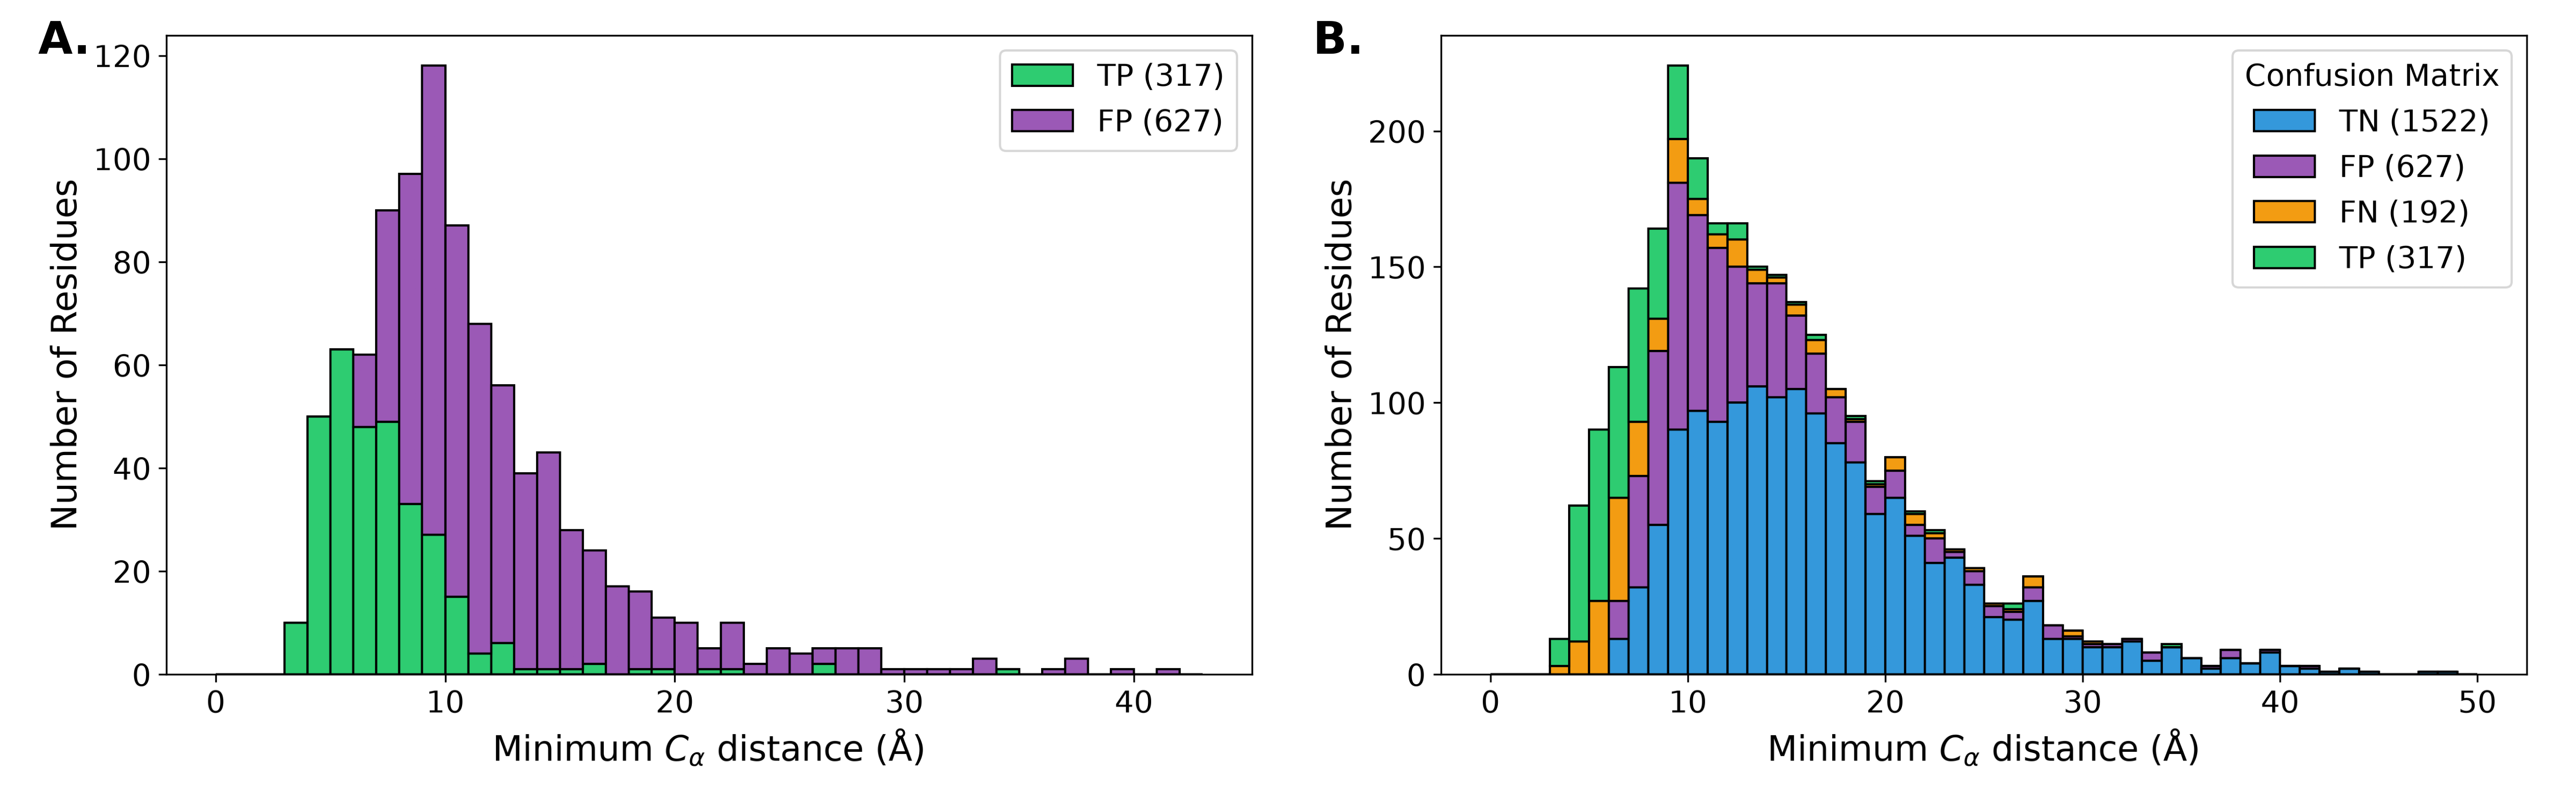
\includegraphics[width=\linewidth]{SF1_hydrolases.png}
\captionsetup{labelformat=empty}
\caption{\textbf{SI Fig. S1. Confusion Matrix Histograms for Hydrolase Receptors}}
\label{fig:sf1_hydrolases}
\end{figure}

\clearpage
% In your document preamble: \usepackage{booktabs}, \usepackage{hyperref}, \usepackage{longtable}, \usepackage{caption}
\scriptsize
\setlength{\tabcolsep}{3pt}
\begin{longtable}{llllrr@{\hspace{0.8cm}}llllrr}
\captionsetup{labelformat=empty}
\caption{\textbf{SI Table S3. Data for Transferase Receptors}}
\label{tab:st3} \\
\toprule
apo\_pdb & holo\_pdb & apo\_bmrb & holo\_bmrb & F1 & MCC & apo\_pdb & holo\_pdb & apo\_bmrb & holo\_bmrb & F1 & MCC \\
\midrule
\endfirsthead
\caption[]{(continued)} \\
\toprule
apo\_pdb & holo\_pdb & apo\_bmrb & holo\_bmrb & F1 & MCC & apo\_pdb & holo\_pdb & apo\_bmrb & holo\_bmrb & F1 & MCC \\
\midrule
\endhead
\bottomrule
\endfoot
\bottomrule
\endlastfoot
 & \href{https://www.rcsb.org/structure/2N9P}{2N9P} & \href{https://bmrb.io/data_library/summary/index.php?bmrbId=25913}{25913} & \href{https://bmrb.io/data_library/summary/index.php?bmrbId=25914}{25914} & 0.72 & 0.57 &  & \href{https://www.rcsb.org/structure/2LGK}{2LGK} & \href{https://bmrb.io/data_library/summary/index.php?bmrbId=17813}{17813} & \href{https://bmrb.io/data_library/summary/index.php?bmrbId=17812}{17812} & 0.52 & 0.24 \\
 & \href{https://www.rcsb.org/structure/2PLD}{2PLD} & \href{https://bmrb.io/data_library/summary/index.php?bmrbId=5318}{5318} & \href{https://bmrb.io/data_library/summary/index.php?bmrbId=5310}{5310} & 0.59 & 0.52 &  & \href{https://www.rcsb.org/structure/2YS5}{2YS5} & \href{https://bmrb.io/data_library/summary/index.php?bmrbId=11095}{11095} & \href{https://bmrb.io/data_library/summary/index.php?bmrbId=11094}{11094} & 0.30 & 0.20 \\
 & \href{https://www.rcsb.org/structure/2K7A}{2K7A} & \href{https://bmrb.io/data_library/summary/index.php?bmrbId=5461}{5461} & \href{https://bmrb.io/data_library/summary/index.php?bmrbId=16809}{16809} & 0.50 & 0.45 & \href{https://www.rcsb.org/structure/1U2N}{1U2N} & \href{https://www.rcsb.org/structure/1R8U}{1R8U} & \href{https://bmrb.io/data_library/summary/index.php?bmrbId=6268}{6268} & \href{https://bmrb.io/data_library/summary/index.php?bmrbId=5987}{5987} & 0.56 & 0.19 \\
\href{https://www.rcsb.org/structure/2LSY}{2LSY} & \href{https://www.rcsb.org/structure/2N1G}{2N1G} & \href{https://bmrb.io/data_library/summary/index.php?bmrbId=18455}{18455} & \href{https://bmrb.io/data_library/summary/index.php?bmrbId=25559}{25559} & 0.53 & 0.44 & \href{https://www.rcsb.org/structure/6VED}{6VED} & \href{https://www.rcsb.org/structure/2L3R}{2L3R} & \href{https://bmrb.io/data_library/summary/index.php?bmrbId=30703}{30703} & \href{https://bmrb.io/data_library/summary/index.php?bmrbId=17200}{17200} & 0.31 & 0.18 \\
 & \href{https://www.rcsb.org/structure/2MOW}{2MOW} & \href{https://bmrb.io/data_library/summary/index.php?bmrbId=17173}{17173} & \href{https://bmrb.io/data_library/summary/index.php?bmrbId=19954}{19954} & 0.41 & 0.43 &  & \href{https://www.rcsb.org/structure/5J8H}{5J8H} & \href{https://bmrb.io/data_library/summary/index.php?bmrbId=51289}{51289} & \href{https://bmrb.io/data_library/summary/index.php?bmrbId=30063}{30063} & 0.43 & 0.17 \\
\href{https://www.rcsb.org/structure/2LSY}{2LSY} & \href{https://www.rcsb.org/structure/2LSK}{2LSK} & \href{https://bmrb.io/data_library/summary/index.php?bmrbId=18455}{18455} & \href{https://bmrb.io/data_library/summary/index.php?bmrbId=18434}{18434} & 0.48 & 0.43 &  & \href{https://www.rcsb.org/structure/2LXS}{2LXS} & \href{https://bmrb.io/data_library/summary/index.php?bmrbId=6095}{6095} & \href{https://bmrb.io/data_library/summary/index.php?bmrbId=18694}{18694} & 0.32 & 0.17 \\
 & \href{https://www.rcsb.org/structure/2LVO}{2LVO} & \href{https://bmrb.io/data_library/summary/index.php?bmrbId=18581}{18581} & \href{https://bmrb.io/data_library/summary/index.php?bmrbId=18582}{18582} & 0.56 & 0.40 &  & \href{https://www.rcsb.org/structure/8SG2}{8SG2} & \href{https://bmrb.io/data_library/summary/index.php?bmrbId=27579}{27579} & \href{https://bmrb.io/data_library/summary/index.php?bmrbId=31080}{31080} & 0.37 & 0.16 \\
\href{https://www.rcsb.org/structure/7JMY}{7JMY} & \href{https://www.rcsb.org/structure/7JYN}{7JYN} & \href{https://bmrb.io/data_library/summary/index.php?bmrbId=30782}{30782} & \href{https://bmrb.io/data_library/summary/index.php?bmrbId=30790}{30790} & 0.51 & 0.40 &  & \href{https://www.rcsb.org/structure/6QXZ}{6QXZ} & \href{https://bmrb.io/data_library/summary/index.php?bmrbId=27250}{27250} & \href{https://bmrb.io/data_library/summary/index.php?bmrbId=27251}{27251} & 0.42 & 0.13 \\
 & \href{https://www.rcsb.org/structure/2OJ2}{2OJ2} & \href{https://bmrb.io/data_library/summary/index.php?bmrbId=4122}{4122} & \href{https://bmrb.io/data_library/summary/index.php?bmrbId=6581}{6581} & 0.42 & 0.37 &  & \href{https://www.rcsb.org/structure/2G35}{2G35} & \href{https://bmrb.io/data_library/summary/index.php?bmrbId=15792}{15792} & \href{https://bmrb.io/data_library/summary/index.php?bmrbId=7061}{7061} & 0.17 & 0.04 \\
 & \href{https://www.rcsb.org/structure/2N8T}{2N8T} & \href{https://bmrb.io/data_library/summary/index.php?bmrbId=25866}{25866} & \href{https://bmrb.io/data_library/summary/index.php?bmrbId=25865}{25865} & 0.61 & 0.37 & \href{https://www.rcsb.org/structure/2JNS}{2JNS} & \href{https://www.rcsb.org/structure/2ND1}{2ND1} & \href{https://bmrb.io/data_library/summary/index.php?bmrbId=15125}{15125} & \href{https://bmrb.io/data_library/summary/index.php?bmrbId=26043}{26043} & 0.11 & 0.02 \\
\href{https://www.rcsb.org/structure/2JNS}{2JNS} & \href{https://www.rcsb.org/structure/2NCZ}{2NCZ} & \href{https://bmrb.io/data_library/summary/index.php?bmrbId=15125}{15125} & \href{https://bmrb.io/data_library/summary/index.php?bmrbId=26041}{26041} & 0.46 & 0.35 &  & \href{https://www.rcsb.org/structure/2LGG}{2LGG} & \href{https://bmrb.io/data_library/summary/index.php?bmrbId=17813}{17813} & \href{https://bmrb.io/data_library/summary/index.php?bmrbId=17808}{17808} & 0.38 & -0.03 \\
 & \href{https://www.rcsb.org/structure/2MC6}{2MC6} & \href{https://bmrb.io/data_library/summary/index.php?bmrbId=19428}{19428} & \href{https://bmrb.io/data_library/summary/index.php?bmrbId=19429}{19429} & 0.46 & 0.33 &  & \href{https://www.rcsb.org/structure/2I94}{2I94} & \href{https://bmrb.io/data_library/summary/index.php?bmrbId=5332}{5332} & \href{https://bmrb.io/data_library/summary/index.php?bmrbId=7293}{7293} & 0.15 & -0.04 \\
\href{https://www.rcsb.org/structure/1W1F}{1W1F} & \href{https://www.rcsb.org/structure/1WA7}{1WA7} & \href{https://bmrb.io/data_library/summary/index.php?bmrbId=6261}{6261} & \href{https://bmrb.io/data_library/summary/index.php?bmrbId=6456}{6456} & 0.48 & 0.32 &  & \href{https://www.rcsb.org/structure/2K8F}{2K8F} & \href{https://bmrb.io/data_library/summary/index.php?bmrbId=34231}{34231} & \href{https://bmrb.io/data_library/summary/index.php?bmrbId=15944}{15944} & 0.16 & -0.08 \\
 & \href{https://www.rcsb.org/structure/5VF0}{5VF0} & \href{https://bmrb.io/data_library/summary/index.php?bmrbId=17769}{17769} & \href{https://bmrb.io/data_library/summary/index.php?bmrbId=30276}{30276} & 0.31 & 0.27 &  & \href{https://www.rcsb.org/structure/9C5E}{9C5E} & \href{https://bmrb.io/data_library/summary/index.php?bmrbId=18642}{18642} & \href{https://bmrb.io/data_library/summary/index.php?bmrbId=31177}{31177} & 0.22 & -0.17 \\
 & \href{https://www.rcsb.org/structure/2KYL}{2KYL} & \href{https://bmrb.io/data_library/summary/index.php?bmrbId=15972}{15972} & \href{https://bmrb.io/data_library/summary/index.php?bmrbId=16967}{16967} & 0.42 & 0.25 &  & \href{https://www.rcsb.org/structure/2JMF}{2JMF} & \href{https://bmrb.io/data_library/summary/index.php?bmrbId=6262}{6262} & \href{https://bmrb.io/data_library/summary/index.php?bmrbId=15016}{15016} & 0.00 & -0.19 \\
 & \href{https://www.rcsb.org/structure/6U19}{6U19} & \href{https://bmrb.io/data_library/summary/index.php?bmrbId=16620}{16620} & \href{https://bmrb.io/data_library/summary/index.php?bmrbId=27875}{27875} & 0.46 & 0.24 &  &  &  &  &  &  \\
\end{longtable}

\begin{figure}[htbp]
\centering
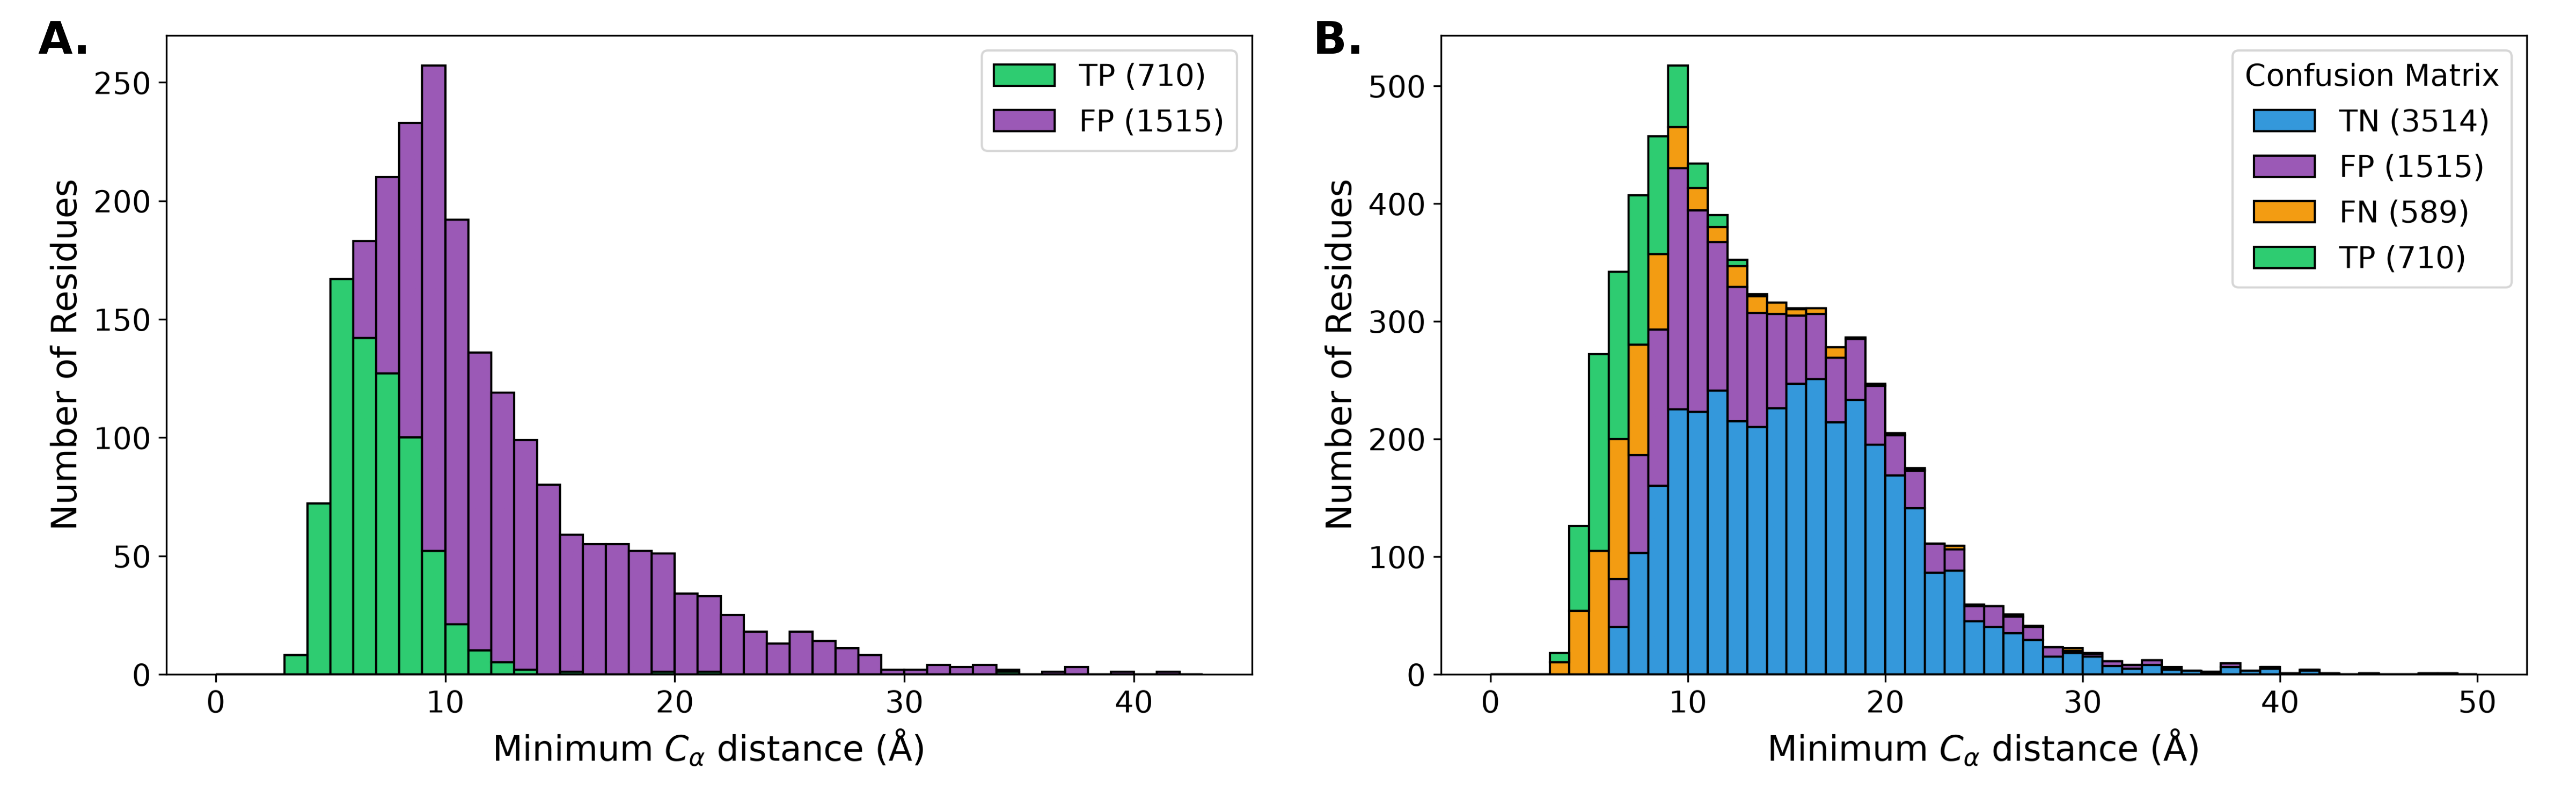
\includegraphics[width=\linewidth]{SF2_transferases.png}
\captionsetup{labelformat=empty}
\caption{\textbf{SI Fig. S2. Confusion Matrix Histograms for Transferase Receptors} ($n=31$)}
\label{fig:sf2_transferases}
\end{figure}

\clearpage

% ST4–ST6 — SCOPe fold classes (+ SF3–SF5)
% In your document preamble: \usepackage{booktabs}, \usepackage{hyperref}, \usepackage{longtable}, \usepackage{caption}
\scriptsize
\setlength{\tabcolsep}{3pt}
\begin{longtable}{llllrr@{\hspace{0.8cm}}llllrr}
\captionsetup{labelformat=empty}
\caption{\textbf{SI Table S4. Data for All Alpha Receptors}}
\label{tab:st4} \\
\toprule
apo\_pdb & holo\_pdb & apo\_bmrb & holo\_bmrb & F1 & MCC & apo\_pdb & holo\_pdb & apo\_bmrb & holo\_bmrb & F1 & MCC \\
\midrule
\endfirsthead
\caption[]{(continued)} \\
\toprule
apo\_pdb & holo\_pdb & apo\_bmrb & holo\_bmrb & F1 & MCC & apo\_pdb & holo\_pdb & apo\_bmrb & holo\_bmrb & F1 & MCC \\
\midrule
\endhead
\bottomrule
\endfoot
\bottomrule
\endlastfoot
 & \href{https://www.rcsb.org/structure/2KSP}{2KSP} & \href{https://bmrb.io/data_library/summary/index.php?bmrbId=15279}{15279} & \href{https://bmrb.io/data_library/summary/index.php?bmrbId=16671}{16671} & 0.53 & 0.44 &  & \href{https://www.rcsb.org/structure/2LXS}{2LXS} & \href{https://bmrb.io/data_library/summary/index.php?bmrbId=6095}{6095} & \href{https://bmrb.io/data_library/summary/index.php?bmrbId=18694}{18694} & 0.32 & 0.17 \\
 & \href{https://www.rcsb.org/structure/6FDP}{6FDP} & \href{https://bmrb.io/data_library/summary/index.php?bmrbId=19757}{19757} & \href{https://bmrb.io/data_library/summary/index.php?bmrbId=34223}{34223} & 0.48 & 0.43 &  & \href{https://www.rcsb.org/structure/1PD7}{1PD7} & \href{https://bmrb.io/data_library/summary/index.php?bmrbId=6899}{6899} & \href{https://bmrb.io/data_library/summary/index.php?bmrbId=5808}{5808} & 0.38 & 0.16 \\
 & \href{https://www.rcsb.org/structure/2L6E}{2L6E} & \href{https://bmrb.io/data_library/summary/index.php?bmrbId=16555}{16555} & \href{https://bmrb.io/data_library/summary/index.php?bmrbId=17307}{17307} & 0.55 & 0.43 &  & \href{https://www.rcsb.org/structure/1ONV}{1ONV} & \href{https://bmrb.io/data_library/summary/index.php?bmrbId=27288}{27288} & \href{https://bmrb.io/data_library/summary/index.php?bmrbId=5685}{5685} & 0.35 & 0.14 \\
 & \href{https://www.rcsb.org/structure/2JXC}{2JXC} & \href{https://bmrb.io/data_library/summary/index.php?bmrbId=4184}{4184} & \href{https://bmrb.io/data_library/summary/index.php?bmrbId=15554}{15554} & 0.60 & 0.39 &  & \href{https://www.rcsb.org/structure/2M0K}{2M0K} & \href{https://bmrb.io/data_library/summary/index.php?bmrbId=51289}{51289} & \href{https://bmrb.io/data_library/summary/index.php?bmrbId=17771}{17771} & 0.42 & 0.14 \\
 & \href{https://www.rcsb.org/structure/6FDT}{6FDT} & \href{https://bmrb.io/data_library/summary/index.php?bmrbId=19757}{19757} & \href{https://bmrb.io/data_library/summary/index.php?bmrbId=34224}{34224} & 0.42 & 0.38 &  & \href{https://www.rcsb.org/structure/2KTB}{2KTB} & \href{https://bmrb.io/data_library/summary/index.php?bmrbId=51472}{51472} & \href{https://bmrb.io/data_library/summary/index.php?bmrbId=16694}{16694} & 0.20 & 0.13 \\
 & \href{https://www.rcsb.org/structure/2LP0}{2LP0} & \href{https://bmrb.io/data_library/summary/index.php?bmrbId=25142}{25142} & \href{https://bmrb.io/data_library/summary/index.php?bmrbId=17407}{17407} & 0.43 & 0.34 &  & \href{https://www.rcsb.org/structure/1SY9}{1SY9} & \href{https://bmrb.io/data_library/summary/index.php?bmrbId=51289}{51289} & \href{https://bmrb.io/data_library/summary/index.php?bmrbId=5480}{5480} & 0.36 & 0.06 \\
 & \href{https://www.rcsb.org/structure/2RQG}{2RQG} & \href{https://bmrb.io/data_library/summary/index.php?bmrbId=4915}{4915} & \href{https://bmrb.io/data_library/summary/index.php?bmrbId=10019}{10019} & 0.44 & 0.32 &  & \href{https://www.rcsb.org/structure/2N80}{2N80} & \href{https://bmrb.io/data_library/summary/index.php?bmrbId=25883}{25883} & \href{https://bmrb.io/data_library/summary/index.php?bmrbId=25829}{25829} & 0.27 & 0.04 \\
 & \href{https://www.rcsb.org/structure/1H8B}{1H8B} & \href{https://bmrb.io/data_library/summary/index.php?bmrbId=17627}{17627} & \href{https://bmrb.io/data_library/summary/index.php?bmrbId=4453}{4453} & 0.33 & 0.24 &  & \href{https://www.rcsb.org/structure/2M0J}{2M0J} & \href{https://bmrb.io/data_library/summary/index.php?bmrbId=51289}{51289} & \href{https://bmrb.io/data_library/summary/index.php?bmrbId=17771}{17771} & 0.35 & 0.02 \\
 & \href{https://www.rcsb.org/structure/2JZI}{2JZI} & \href{https://bmrb.io/data_library/summary/index.php?bmrbId=51289}{51289} & \href{https://bmrb.io/data_library/summary/index.php?bmrbId=15624}{15624} & 0.43 & 0.22 &  & \href{https://www.rcsb.org/structure/2I94}{2I94} & \href{https://bmrb.io/data_library/summary/index.php?bmrbId=5332}{5332} & \href{https://bmrb.io/data_library/summary/index.php?bmrbId=7293}{7293} & 0.15 & -0.04 \\
 & \href{https://www.rcsb.org/structure/5J8H}{5J8H} & \href{https://bmrb.io/data_library/summary/index.php?bmrbId=51289}{51289} & \href{https://bmrb.io/data_library/summary/index.php?bmrbId=30063}{30063} & 0.43 & 0.17 &  & \href{https://www.rcsb.org/structure/2MES}{2MES} & \href{https://bmrb.io/data_library/summary/index.php?bmrbId=51289}{51289} & \href{https://bmrb.io/data_library/summary/index.php?bmrbId=19238}{19238} & 0.30 & -0.05 \\
\end{longtable}

\begin{figure}[htbp]
\centering
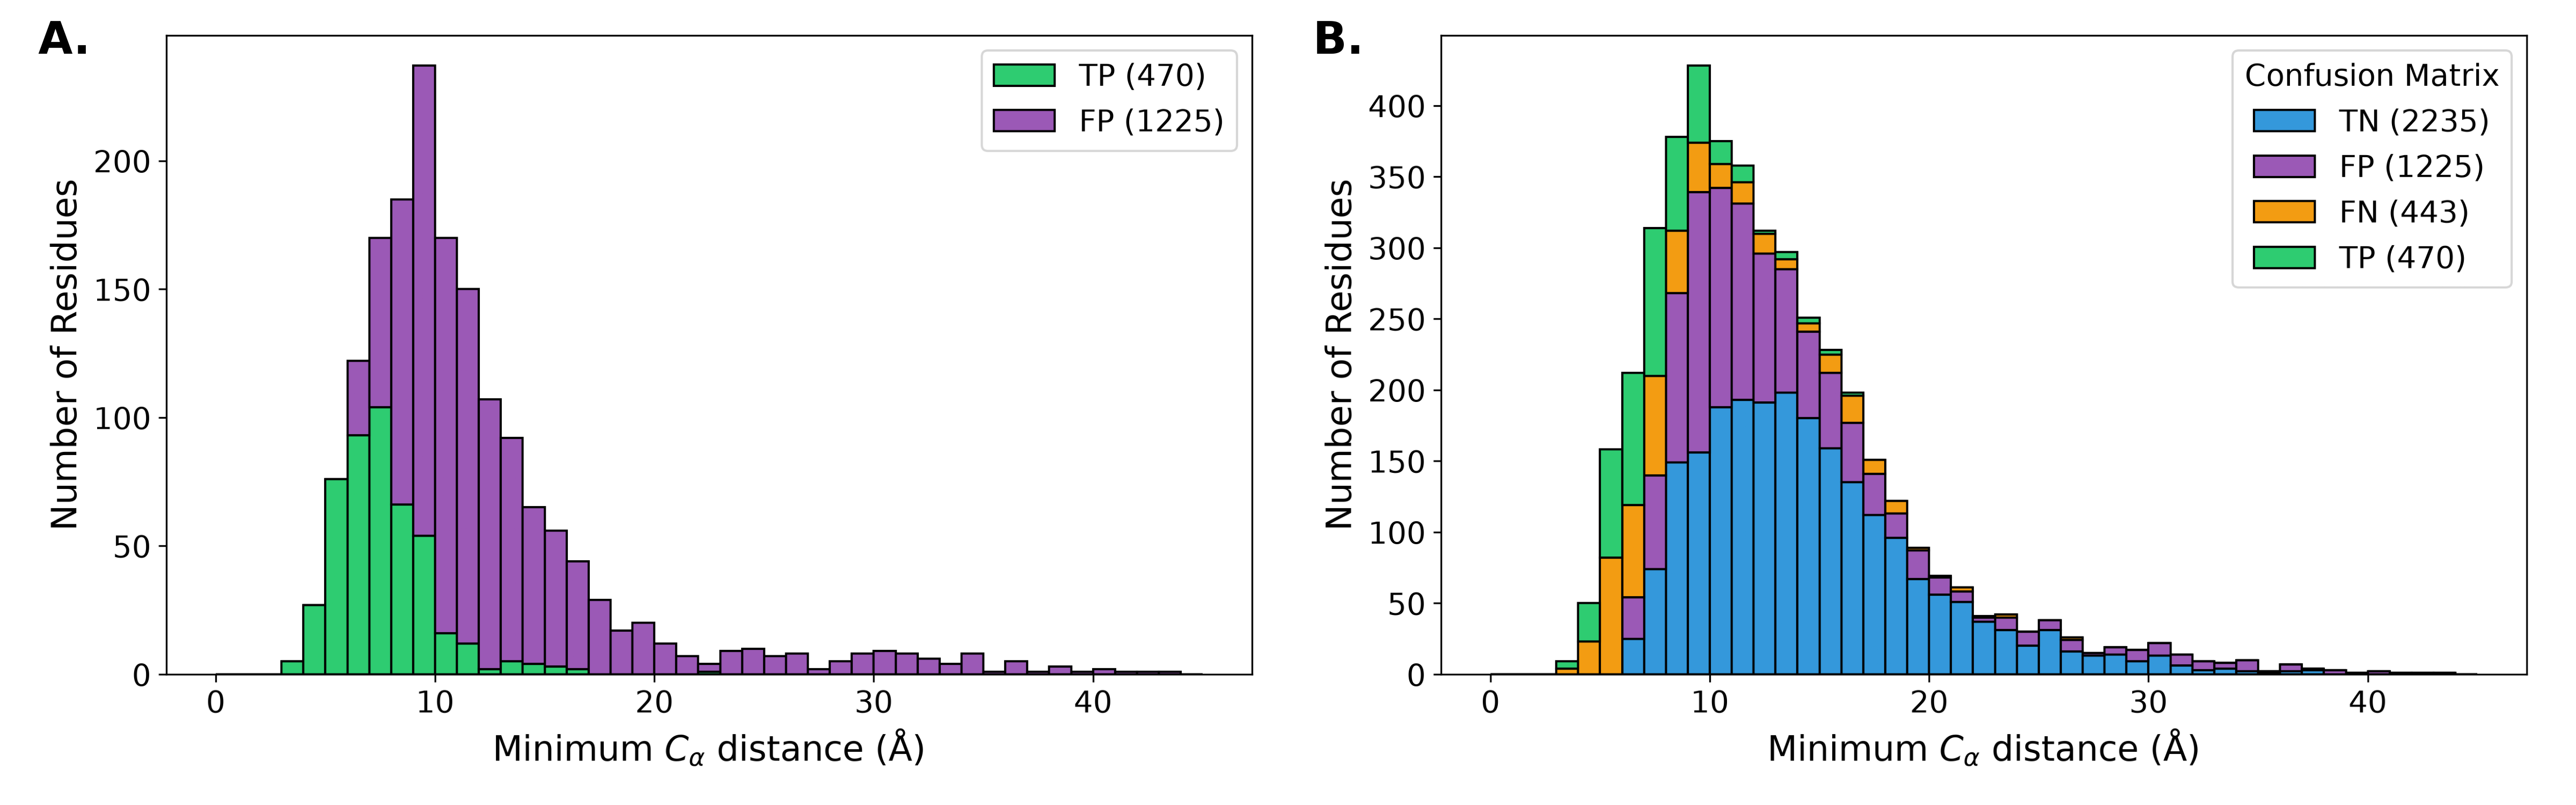
\includegraphics[width=\linewidth]{SF3_all_alpha_proteins.png}
\captionsetup{labelformat=empty}
\caption{\textbf{SI Fig. S3. Confusion Matrix Histograms for All Alpha Receptors} ($n=20$)}
\label{fig:sf3_all_alpha_proteins}
\end{figure}

\clearpage
% In your document preamble: \usepackage{booktabs}, \usepackage{hyperref}, \usepackage{longtable}, \usepackage{caption}
\scriptsize
\setlength{\tabcolsep}{3pt}
\begin{longtable}{llllrr@{\hspace{0.8cm}}llllrr}
\captionsetup{labelformat=empty}
\caption{\textbf{SI Table S5. Data for All Beta Receptors}}
\label{tab:st5} \\
\toprule
apo\_pdb & holo\_pdb & apo\_bmrb & holo\_bmrb & F1 & MCC & apo\_pdb & holo\_pdb & apo\_bmrb & holo\_bmrb & F1 & MCC \\
\midrule
\endfirsthead
\caption[]{(continued)} \\
\toprule
apo\_pdb & holo\_pdb & apo\_bmrb & holo\_bmrb & F1 & MCC & apo\_pdb & holo\_pdb & apo\_bmrb & holo\_bmrb & F1 & MCC \\
\midrule
\endhead
\bottomrule
\endfoot
\bottomrule
\endlastfoot
 & \href{https://www.rcsb.org/structure/1YWI}{1YWI} & \href{https://bmrb.io/data_library/summary/index.php?bmrbId=6558}{6558} & \href{https://bmrb.io/data_library/summary/index.php?bmrbId=6559}{6559} & 0.78 & 0.72 & \href{https://www.rcsb.org/structure/2GS0}{2GS0} & \href{https://www.rcsb.org/structure/2MKR}{2MKR} & \href{https://bmrb.io/data_library/summary/index.php?bmrbId=6225}{6225} & \href{https://bmrb.io/data_library/summary/index.php?bmrbId=19791}{19791} & 0.30 & 0.29 \\
 & \href{https://www.rcsb.org/structure/2MCN}{2MCN} & \href{https://bmrb.io/data_library/summary/index.php?bmrbId=16641}{16641} & \href{https://bmrb.io/data_library/summary/index.php?bmrbId=19447}{19447} & 0.79 & 0.71 & \href{https://www.rcsb.org/structure/1SSF}{1SSF} & \href{https://www.rcsb.org/structure/2LVM}{2LVM} & \href{https://bmrb.io/data_library/summary/index.php?bmrbId=5878}{5878} & \href{https://bmrb.io/data_library/summary/index.php?bmrbId=18579}{18579} & 0.33 & 0.28 \\
 & \href{https://www.rcsb.org/structure/2MCN}{2MCN} & \href{https://bmrb.io/data_library/summary/index.php?bmrbId=6457}{6457} & \href{https://bmrb.io/data_library/summary/index.php?bmrbId=19447}{19447} & 0.76 & 0.67 &  & \href{https://www.rcsb.org/structure/2M3M}{2M3M} & \href{https://bmrb.io/data_library/summary/index.php?bmrbId=17373}{17373} & \href{https://bmrb.io/data_library/summary/index.php?bmrbId=17942}{17942} & 0.44 & 0.26 \\
 & \href{https://www.rcsb.org/structure/2AFF}{2AFF} & \href{https://bmrb.io/data_library/summary/index.php?bmrbId=5959}{5959} & \href{https://bmrb.io/data_library/summary/index.php?bmrbId=6748}{6748} & 0.67 & 0.53 & \href{https://www.rcsb.org/structure/7QCX}{7QCX} & \href{https://www.rcsb.org/structure/1D5G}{1D5G} & \href{https://bmrb.io/data_library/summary/index.php?bmrbId=34688}{34688} & \href{https://bmrb.io/data_library/summary/index.php?bmrbId=4516}{4516} & 0.27 & 0.26 \\
 & \href{https://www.rcsb.org/structure/5I22}{5I22} & \href{https://bmrb.io/data_library/summary/index.php?bmrbId=4871}{4871} & \href{https://bmrb.io/data_library/summary/index.php?bmrbId=30010}{30010} & 0.56 & 0.50 &  & \href{https://www.rcsb.org/structure/2RVB}{2RVB} & \href{https://bmrb.io/data_library/summary/index.php?bmrbId=4901}{4901} & \href{https://bmrb.io/data_library/summary/index.php?bmrbId=11594}{11594} & 0.45 & 0.23 \\
 & \href{https://www.rcsb.org/structure/2ROZ}{2ROZ} & \href{https://bmrb.io/data_library/summary/index.php?bmrbId=10235}{10235} & \href{https://bmrb.io/data_library/summary/index.php?bmrbId=10236}{10236} & 0.59 & 0.50 &  & \href{https://www.rcsb.org/structure/2L4T}{2L4T} & \href{https://bmrb.io/data_library/summary/index.php?bmrbId=17254}{17254} & \href{https://bmrb.io/data_library/summary/index.php?bmrbId=17255}{17255} & 0.31 & 0.22 \\
\href{https://www.rcsb.org/structure/2GS0}{2GS0} & \href{https://www.rcsb.org/structure/2LOX}{2LOX} & \href{https://bmrb.io/data_library/summary/index.php?bmrbId=6225}{6225} & \href{https://bmrb.io/data_library/summary/index.php?bmrbId=18229}{18229} & 0.55 & 0.49 &  & \href{https://www.rcsb.org/structure/1I5H}{1I5H} & \href{https://bmrb.io/data_library/summary/index.php?bmrbId=26698}{26698} & \href{https://bmrb.io/data_library/summary/index.php?bmrbId=4963}{4963} & 0.40 & 0.20 \\
\href{https://www.rcsb.org/structure/2GS0}{2GS0} & \href{https://www.rcsb.org/structure/2N0Y}{2N0Y} & \href{https://bmrb.io/data_library/summary/index.php?bmrbId=6225}{6225} & \href{https://bmrb.io/data_library/summary/index.php?bmrbId=25540}{25540} & 0.50 & 0.47 &  & \href{https://www.rcsb.org/structure/2LOZ}{2LOZ} & \href{https://bmrb.io/data_library/summary/index.php?bmrbId=10318}{10318} & \href{https://bmrb.io/data_library/summary/index.php?bmrbId=17364}{17364} & 0.31 & 0.19 \\
\href{https://www.rcsb.org/structure/2GS0}{2GS0} & \href{https://www.rcsb.org/structure/2M14}{2M14} & \href{https://bmrb.io/data_library/summary/index.php?bmrbId=6225}{6225} & \href{https://bmrb.io/data_library/summary/index.php?bmrbId=18842}{18842} & 0.41 & 0.42 &  & \href{https://www.rcsb.org/structure/2FIN}{2FIN} & \href{https://bmrb.io/data_library/summary/index.php?bmrbId=6809}{6809} & \href{https://bmrb.io/data_library/summary/index.php?bmrbId=7024}{7024} & 0.19 & 0.19 \\
\href{https://www.rcsb.org/structure/2GS0}{2GS0} & \href{https://www.rcsb.org/structure/2N23}{2N23} & \href{https://bmrb.io/data_library/summary/index.php?bmrbId=6225}{6225} & \href{https://bmrb.io/data_library/summary/index.php?bmrbId=25584}{25584} & 0.40 & 0.42 & \href{https://www.rcsb.org/structure/2GS0}{2GS0} & \href{https://www.rcsb.org/structure/5URN}{5URN} & \href{https://bmrb.io/data_library/summary/index.php?bmrbId=6225}{6225} & \href{https://bmrb.io/data_library/summary/index.php?bmrbId=30243}{30243} & 0.27 & 0.19 \\
\href{https://www.rcsb.org/structure/2RQT}{2RQT} & \href{https://www.rcsb.org/structure/2RQU}{2RQU} & \href{https://bmrb.io/data_library/summary/index.php?bmrbId=11081}{11081} & \href{https://bmrb.io/data_library/summary/index.php?bmrbId=11082}{11082} & 0.60 & 0.41 &  & \href{https://www.rcsb.org/structure/2NMB}{2NMB} & \href{https://bmrb.io/data_library/summary/index.php?bmrbId=4683}{4683} & \href{https://bmrb.io/data_library/summary/index.php?bmrbId=4263}{4263} & 0.19 & 0.17 \\
 & \href{https://www.rcsb.org/structure/1N7T}{1N7T} & \href{https://bmrb.io/data_library/summary/index.php?bmrbId=18785}{18785} & \href{https://bmrb.io/data_library/summary/index.php?bmrbId=5631}{5631} & 0.45 & 0.40 &  & \href{https://www.rcsb.org/structure/1VJ6}{1VJ6} & \href{https://bmrb.io/data_library/summary/index.php?bmrbId=5131}{5131} & \href{https://bmrb.io/data_library/summary/index.php?bmrbId=6060}{6060} & 0.30 & 0.16 \\
 & \href{https://www.rcsb.org/structure/1DDM}{1DDM} & \href{https://bmrb.io/data_library/summary/index.php?bmrbId=4683}{4683} & \href{https://bmrb.io/data_library/summary/index.php?bmrbId=4263}{4263} & 0.33 & 0.35 &  & \href{https://www.rcsb.org/structure/5XV8}{5XV8} & \href{https://bmrb.io/data_library/summary/index.php?bmrbId=4901}{4901} & \href{https://bmrb.io/data_library/summary/index.php?bmrbId=36101}{36101} & 0.40 & 0.15 \\
 & \href{https://www.rcsb.org/structure/2KPL}{2KPL} & \href{https://bmrb.io/data_library/summary/index.php?bmrbId=6911}{6911} & \href{https://bmrb.io/data_library/summary/index.php?bmrbId=16559}{16559} & 0.43 & 0.35 &  & \href{https://www.rcsb.org/structure/2HUG}{2HUG} & \href{https://bmrb.io/data_library/summary/index.php?bmrbId=6592}{6592} & \href{https://bmrb.io/data_library/summary/index.php?bmrbId=7241}{7241} & 0.38 & 0.14 \\
 & \href{https://www.rcsb.org/structure/2MS4}{2MS4} & \href{https://bmrb.io/data_library/summary/index.php?bmrbId=2208}{2208} & \href{https://bmrb.io/data_library/summary/index.php?bmrbId=25104}{25104} & 0.33 & 0.33 & \href{https://www.rcsb.org/structure/2KQ3}{2KQ3} & \href{https://www.rcsb.org/structure/2KHS}{2KHS} & \href{https://bmrb.io/data_library/summary/index.php?bmrbId=16585}{16585} & \href{https://bmrb.io/data_library/summary/index.php?bmrbId=15357}{15357} & 0.34 & 0.13 \\
\href{https://www.rcsb.org/structure/1W1F}{1W1F} & \href{https://www.rcsb.org/structure/1WA7}{1WA7} & \href{https://bmrb.io/data_library/summary/index.php?bmrbId=6261}{6261} & \href{https://bmrb.io/data_library/summary/index.php?bmrbId=6456}{6456} & 0.48 & 0.32 &  & \href{https://www.rcsb.org/structure/2KOH}{2KOH} & \href{https://bmrb.io/data_library/summary/index.php?bmrbId=27205}{27205} & \href{https://bmrb.io/data_library/summary/index.php?bmrbId=16507}{16507} & 0.26 & 0.06 \\
 & \href{https://www.rcsb.org/structure/2KVQ}{2KVQ} & \href{https://bmrb.io/data_library/summary/index.php?bmrbId=15490}{15490} & \href{https://bmrb.io/data_library/summary/index.php?bmrbId=16788}{16788} & 0.27 & 0.31 &  & \href{https://www.rcsb.org/structure/2G35}{2G35} & \href{https://bmrb.io/data_library/summary/index.php?bmrbId=15792}{15792} & \href{https://bmrb.io/data_library/summary/index.php?bmrbId=7061}{7061} & 0.17 & 0.04 \\
 & \href{https://www.rcsb.org/structure/2FFK}{2FFK} & \href{https://bmrb.io/data_library/summary/index.php?bmrbId=6809}{6809} & \href{https://bmrb.io/data_library/summary/index.php?bmrbId=7024}{7024} & 0.30 & 0.31 &  & \href{https://www.rcsb.org/structure/2KVM}{2KVM} & \href{https://bmrb.io/data_library/summary/index.php?bmrbId=15674}{15674} & \href{https://bmrb.io/data_library/summary/index.php?bmrbId=16778}{16778} & 0.33 & -0.07 \\
 & \href{https://www.rcsb.org/structure/2M0U}{2M0U} & \href{https://bmrb.io/data_library/summary/index.php?bmrbId=18824}{18824} & \href{https://bmrb.io/data_library/summary/index.php?bmrbId=18825}{18825} & 0.35 & 0.31 &  & \href{https://www.rcsb.org/structure/2MNU}{2MNU} & \href{https://bmrb.io/data_library/summary/index.php?bmrbId=4283}{4283} & \href{https://bmrb.io/data_library/summary/index.php?bmrbId=19906}{19906} & 0.15 & -0.09 \\
 & \href{https://www.rcsb.org/structure/2L29}{2L29} & \href{https://bmrb.io/data_library/summary/index.php?bmrbId=17128}{17128} & \href{https://bmrb.io/data_library/summary/index.php?bmrbId=17127}{17127} & 0.27 & 0.30 &  & \href{https://www.rcsb.org/structure/2JMF}{2JMF} & \href{https://bmrb.io/data_library/summary/index.php?bmrbId=6262}{6262} & \href{https://bmrb.io/data_library/summary/index.php?bmrbId=15016}{15016} & 0.00 & -0.19 \\
 & \href{https://www.rcsb.org/structure/2RUK}{2RUK} & \href{https://bmrb.io/data_library/summary/index.php?bmrbId=4901}{4901} & \href{https://bmrb.io/data_library/summary/index.php?bmrbId=11578}{11578} & 0.44 & 0.30 &  &  &  &  &  &  \\
\end{longtable}

\begin{figure}[htbp]
\centering
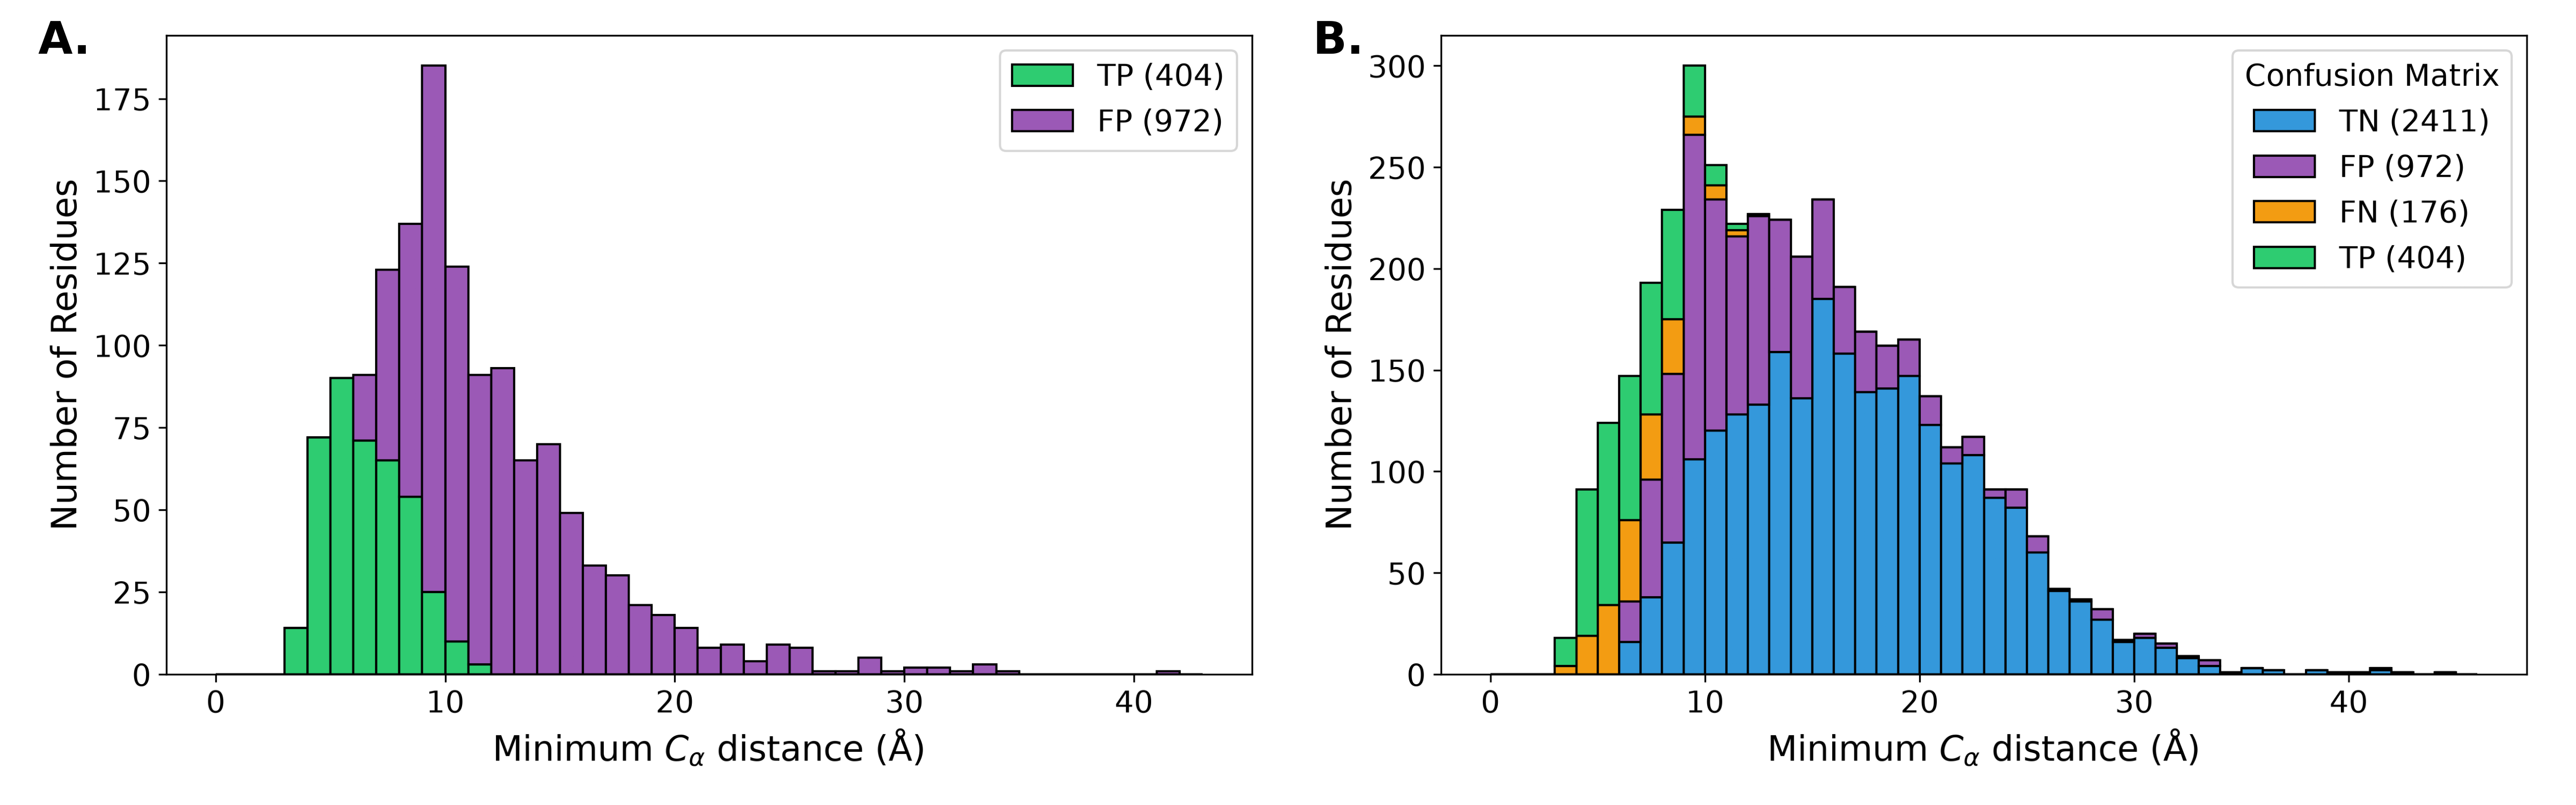
\includegraphics[width=\linewidth]{SF4_all_beta_proteins.png}
\captionsetup{labelformat=empty}
\caption{\textbf{SI Fig. S4. Confusion Matrix Histograms for All Beta Receptors} ($n=41$)}
\label{fig:sf4_all_beta_proteins}
\end{figure}

\clearpage
% In your document preamble: \usepackage{booktabs}, \usepackage{hyperref}, \usepackage{longtable}, \usepackage{caption}
\scriptsize
\setlength{\tabcolsep}{3pt}
\begin{longtable}{llllrr@{\hspace{0.8cm}}llllrr}
\captionsetup{labelformat=empty}
\caption{\textbf{SI Table S6. Data for Alpha and Beta (a+b) Receptors}}
\label{tab:st6} \\
\toprule
apo\_pdb & holo\_pdb & apo\_bmrb & holo\_bmrb & F1 & MCC & apo\_pdb & holo\_pdb & apo\_bmrb & holo\_bmrb & F1 & MCC \\
\midrule
\endfirsthead
\caption[]{(continued)} \\
\toprule
apo\_pdb & holo\_pdb & apo\_bmrb & holo\_bmrb & F1 & MCC & apo\_pdb & holo\_pdb & apo\_bmrb & holo\_bmrb & F1 & MCC \\
\midrule
\endhead
\bottomrule
\endfoot
\bottomrule
\endlastfoot
 & \href{https://www.rcsb.org/structure/2M0G}{2M0G} & \href{https://bmrb.io/data_library/summary/index.php?bmrbId=18802}{18802} & \href{https://bmrb.io/data_library/summary/index.php?bmrbId=18808}{18808} & 0.48 & 0.52 &  & \href{https://www.rcsb.org/structure/2K6Q}{2K6Q} & \href{https://bmrb.io/data_library/summary/index.php?bmrbId=5958}{5958} & \href{https://bmrb.io/data_library/summary/index.php?bmrbId=15877}{15877} & 0.37 & 0.26 \\
 & \href{https://www.rcsb.org/structure/2PLD}{2PLD} & \href{https://bmrb.io/data_library/summary/index.php?bmrbId=5318}{5318} & \href{https://bmrb.io/data_library/summary/index.php?bmrbId=5310}{5310} & 0.59 & 0.52 &  & \href{https://www.rcsb.org/structure/6H8C}{6H8C} & \href{https://bmrb.io/data_library/summary/index.php?bmrbId=18827}{18827} & \href{https://bmrb.io/data_library/summary/index.php?bmrbId=34307}{34307} & 0.31 & 0.23 \\
 & \href{https://www.rcsb.org/structure/2LI5}{2LI5} & \href{https://bmrb.io/data_library/summary/index.php?bmrbId=16835}{16835} & \href{https://bmrb.io/data_library/summary/index.php?bmrbId=17879}{17879} & 0.57 & 0.51 &  & \href{https://www.rcsb.org/structure/1KLQ}{1KLQ} & \href{https://bmrb.io/data_library/summary/index.php?bmrbId=52275}{52275} & \href{https://bmrb.io/data_library/summary/index.php?bmrbId=5299}{5299} & 0.33 & 0.23 \\
 & \href{https://www.rcsb.org/structure/2K7A}{2K7A} & \href{https://bmrb.io/data_library/summary/index.php?bmrbId=5461}{5461} & \href{https://bmrb.io/data_library/summary/index.php?bmrbId=16809}{16809} & 0.50 & 0.45 &  & \href{https://www.rcsb.org/structure/2MUR}{2MUR} & \href{https://bmrb.io/data_library/summary/index.php?bmrbId=25229}{25229} & \href{https://bmrb.io/data_library/summary/index.php?bmrbId=25230}{25230} & 0.57 & 0.23 \\
 & \href{https://www.rcsb.org/structure/2M0G}{2M0G} & \href{https://bmrb.io/data_library/summary/index.php?bmrbId=19034}{19034} & \href{https://bmrb.io/data_library/summary/index.php?bmrbId=18808}{18808} & 0.44 & 0.33 &  & \href{https://www.rcsb.org/structure/2N55}{2N55} & \href{https://bmrb.io/data_library/summary/index.php?bmrbId=52209}{52209} & \href{https://bmrb.io/data_library/summary/index.php?bmrbId=25694}{25694} & 0.24 & -0.12 \\
 & \href{https://www.rcsb.org/structure/2MUR}{2MUR} & \href{https://bmrb.io/data_library/summary/index.php?bmrbId=17769}{17769} & \href{https://bmrb.io/data_library/summary/index.php?bmrbId=25230}{25230} & 0.40 & 0.30 &  & \href{https://www.rcsb.org/structure/2K6D}{2K6D} & \href{https://bmrb.io/data_library/summary/index.php?bmrbId=52081}{52081} & \href{https://bmrb.io/data_library/summary/index.php?bmrbId=15866}{15866} & 0.08 & -0.19 \\
 & \href{https://www.rcsb.org/structure/5VF0}{5VF0} & \href{https://bmrb.io/data_library/summary/index.php?bmrbId=17769}{17769} & \href{https://bmrb.io/data_library/summary/index.php?bmrbId=30276}{30276} & 0.31 & 0.27 &  &  &  &  &  &  \\
\end{longtable}

\begin{figure}[htbp]
\centering
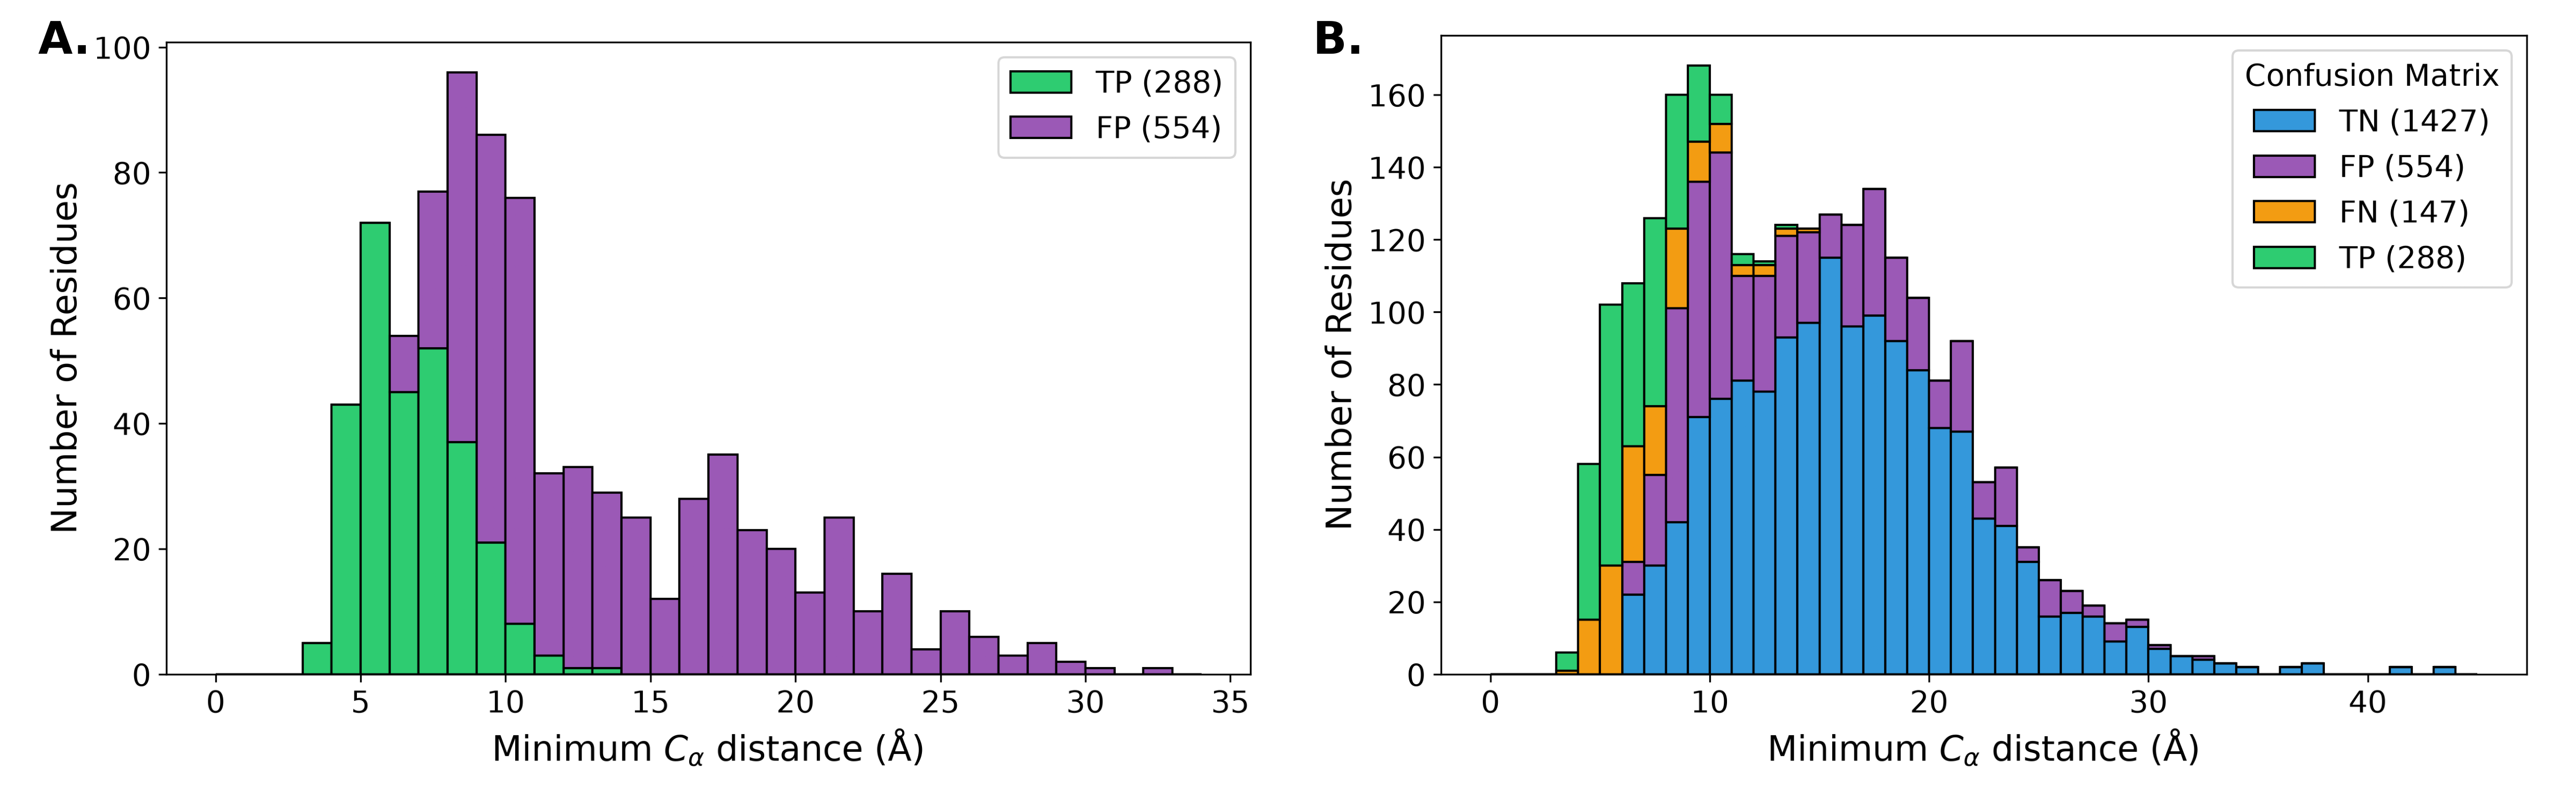
\includegraphics[width=\linewidth]{SF5_alpha_and_beta_proteins_a_plus_b.png}
\captionsetup{labelformat=empty}
\caption{\textbf{SI Fig. S5. Confusion Matrix Histograms for Alpha and Beta (a+b) Receptors} ($n=13$)}
\label{fig:sf5_alpha_and_beta_proteins_a_plus_b}
\end{figure}

\clearpage

% ST7–ST9 — domain selections (+ SF6–SF8)
% In your document preamble: \usepackage{booktabs}, \usepackage{hyperref}, \usepackage{longtable}, \usepackage{caption}
\scriptsize
\setlength{\tabcolsep}{3pt}
\begin{longtable}{llllrr@{\hspace{0.8cm}}llllrr}
\captionsetup{labelformat=empty}
\caption{\textbf{SI Table S7. Data for BET-ET Domain Receptors}}
\label{tab:st7} \\
\toprule
apo\_pdb & holo\_pdb & apo\_bmrb & holo\_bmrb & F1 & MCC & apo\_pdb & holo\_pdb & apo\_bmrb & holo\_bmrb & F1 & MCC \\
\midrule
\endfirsthead
\caption[]{(continued)} \\
\toprule
apo\_pdb & holo\_pdb & apo\_bmrb & holo\_bmrb & F1 & MCC & apo\_pdb & holo\_pdb & apo\_bmrb & holo\_bmrb & F1 & MCC \\
\midrule
\endhead
\bottomrule
\endfoot
\bottomrule
\endlastfoot
\href{https://www.rcsb.org/structure/7JMY}{7JMY} & \href{https://www.rcsb.org/structure/7JYN}{7JYN} & \href{https://bmrb.io/data_library/summary/index.php?bmrbId=30782}{30782} & \href{https://bmrb.io/data_library/summary/index.php?bmrbId=30790}{30790} & 0.53 & 0.43 & \href{https://www.rcsb.org/structure/2JNS}{2JNS} & \href{https://www.rcsb.org/structure/2NCZ}{2NCZ} & \href{https://bmrb.io/data_library/summary/index.php?bmrbId=15125}{15125} & \href{https://bmrb.io/data_library/summary/index.php?bmrbId=26041}{26041} & 0.40 & 0.25 \\
\href{https://www.rcsb.org/structure/7JMY}{7JMY} & \href{https://www.rcsb.org/structure/7JYZ}{7JYZ} & \href{https://bmrb.io/data_library/summary/index.php?bmrbId=30782}{30782} & \href{https://bmrb.io/data_library/summary/index.php?bmrbId=30791}{30791} & 0.50 & 0.40 & \href{https://www.rcsb.org/structure/2JNS}{2JNS} & \href{https://www.rcsb.org/structure/2ND0}{2ND0} & \href{https://bmrb.io/data_library/summary/index.php?bmrbId=15125}{15125} & \href{https://bmrb.io/data_library/summary/index.php?bmrbId=26042}{26042} & 0.31 & 0.09 \\
\href{https://www.rcsb.org/structure/7JMY}{7JMY} & \href{https://www.rcsb.org/structure/7JQ8}{7JQ8} & \href{https://bmrb.io/data_library/summary/index.php?bmrbId=30782}{30782} & \href{https://bmrb.io/data_library/summary/index.php?bmrbId=30786}{30786} & 0.51 & 0.37 & \href{https://www.rcsb.org/structure/2JNS}{2JNS} & \href{https://www.rcsb.org/structure/2ND1}{2ND1} & \href{https://bmrb.io/data_library/summary/index.php?bmrbId=15125}{15125} & \href{https://bmrb.io/data_library/summary/index.php?bmrbId=26043}{26043} & 0.23 & -0.06 \\
\href{https://www.rcsb.org/structure/2JNS}{2JNS} & \href{https://www.rcsb.org/structure/6BNH}{6BNH} & \href{https://bmrb.io/data_library/summary/index.php?bmrbId=15125}{15125} & \href{https://bmrb.io/data_library/summary/index.php?bmrbId=30373}{30373} & 0.48 & 0.36 & \href{https://www.rcsb.org/structure/2JNS}{2JNS} & \href{https://www.rcsb.org/structure/6BGG}{6BGG} & \href{https://bmrb.io/data_library/summary/index.php?bmrbId=15125}{15125} & \href{https://bmrb.io/data_library/summary/index.php?bmrbId=30367}{30367} & 0.14 & -0.08 \\
\end{longtable}

\begin{figure}[htbp]
\centering
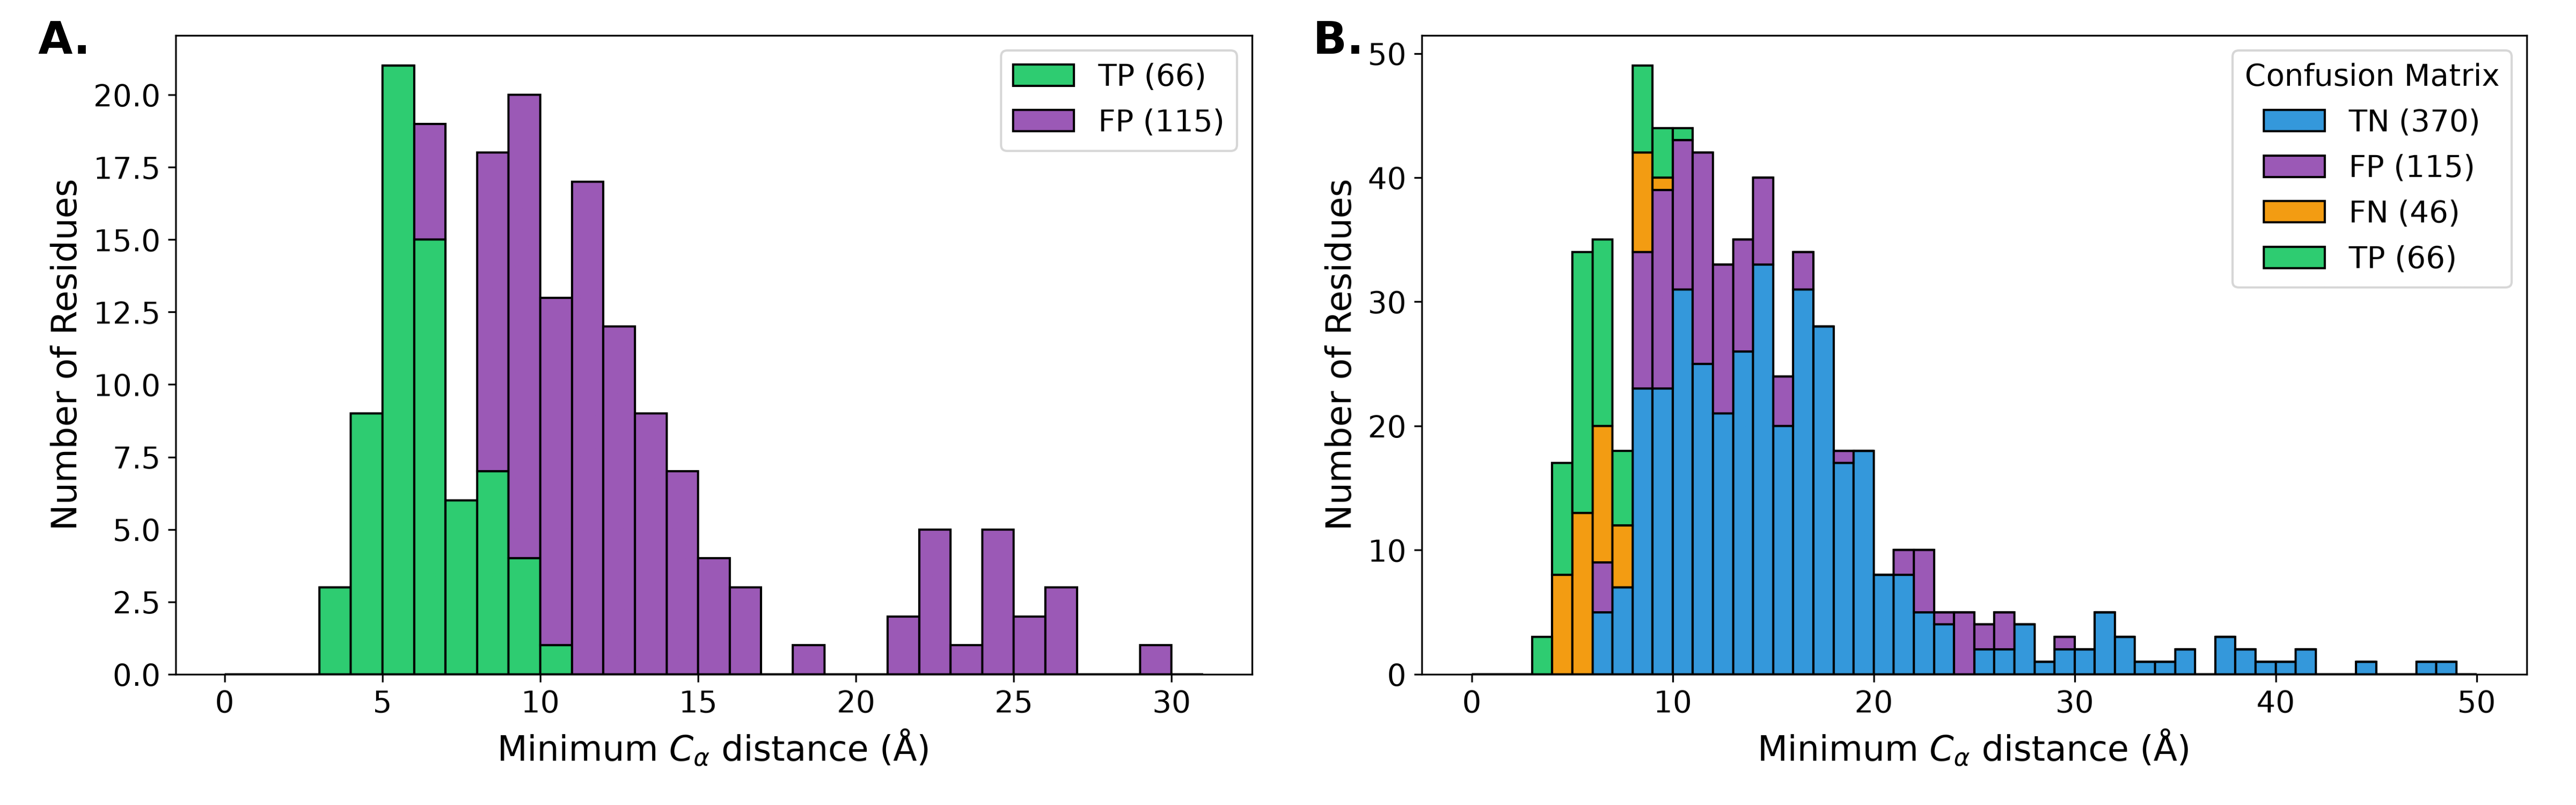
\includegraphics[width=\linewidth]{SF6_BET_ET.png}
\captionsetup{labelformat=empty}
\caption{\textbf{SI Fig. S6. Confusion Matrix Histograms for BET-ET Domain Receptors}}
\label{fig:sf6_bet_et}
\end{figure}

\clearpage
% In your document preamble: \usepackage{booktabs}, \usepackage{hyperref}, \usepackage{longtable}, \usepackage{caption}
\scriptsize
\setlength{\tabcolsep}{3pt}
\begin{longtable}{llllrr@{\hspace{0.8cm}}llllrr}
\captionsetup{labelformat=empty}
\caption{\textbf{SI Table S8. Data for TFIIH Domain Receptors}}
\label{tab:st8} \\
\toprule
apo\_pdb & holo\_pdb & apo\_bmrb & holo\_bmrb & F1 & MCC & apo\_pdb & holo\_pdb & apo\_bmrb & holo\_bmrb & F1 & MCC \\
\midrule
\endfirsthead
\caption[]{(continued)} \\
\toprule
apo\_pdb & holo\_pdb & apo\_bmrb & holo\_bmrb & F1 & MCC & apo\_pdb & holo\_pdb & apo\_bmrb & holo\_bmrb & F1 & MCC \\
\midrule
\endhead
\bottomrule
\endfoot
\bottomrule
\endlastfoot
\href{https://www.rcsb.org/structure/2GS0}{2GS0} & \href{https://www.rcsb.org/structure/2LOX}{2LOX} & \href{https://bmrb.io/data_library/summary/index.php?bmrbId=6225}{6225} & \href{https://bmrb.io/data_library/summary/index.php?bmrbId=18229}{18229} & 0.47 & 0.42 & \href{https://www.rcsb.org/structure/2GS0}{2GS0} & \href{https://www.rcsb.org/structure/5URN}{5URN} & \href{https://bmrb.io/data_library/summary/index.php?bmrbId=6225}{6225} & \href{https://bmrb.io/data_library/summary/index.php?bmrbId=30243}{30243} & 0.29 & 0.23 \\
\href{https://www.rcsb.org/structure/2GS0}{2GS0} & \href{https://www.rcsb.org/structure/2MKR}{2MKR} & \href{https://bmrb.io/data_library/summary/index.php?bmrbId=6225}{6225} & \href{https://bmrb.io/data_library/summary/index.php?bmrbId=19791}{19791} & 0.29 & 0.33 & \href{https://www.rcsb.org/structure/2GS0}{2GS0} & \href{https://www.rcsb.org/structure/2N23}{2N23} & \href{https://bmrb.io/data_library/summary/index.php?bmrbId=6225}{6225} & \href{https://bmrb.io/data_library/summary/index.php?bmrbId=25584}{25584} & 0.17 & 0.22 \\
\href{https://www.rcsb.org/structure/2GS0}{2GS0} & \href{https://www.rcsb.org/structure/2N0Y}{2N0Y} & \href{https://bmrb.io/data_library/summary/index.php?bmrbId=6225}{6225} & \href{https://bmrb.io/data_library/summary/index.php?bmrbId=25540}{25540} & 0.37 & 0.33 &  & \href{https://www.rcsb.org/structure/2RVB}{2RVB} & \href{https://bmrb.io/data_library/summary/index.php?bmrbId=4901}{4901} & \href{https://bmrb.io/data_library/summary/index.php?bmrbId=11594}{11594} & 0.44 & 0.20 \\
 & \href{https://www.rcsb.org/structure/2RUK}{2RUK} & \href{https://bmrb.io/data_library/summary/index.php?bmrbId=4901}{4901} & \href{https://bmrb.io/data_library/summary/index.php?bmrbId=11578}{11578} & 0.44 & 0.30 &  & \href{https://www.rcsb.org/structure/5XV8}{5XV8} & \href{https://bmrb.io/data_library/summary/index.php?bmrbId=4901}{4901} & \href{https://bmrb.io/data_library/summary/index.php?bmrbId=36101}{36101} & 0.37 & 0.09 \\
\href{https://www.rcsb.org/structure/2GS0}{2GS0} & \href{https://www.rcsb.org/structure/2M14}{2M14} & \href{https://bmrb.io/data_library/summary/index.php?bmrbId=6225}{6225} & \href{https://bmrb.io/data_library/summary/index.php?bmrbId=18842}{18842} & 0.24 & 0.23 &  &  &  &  &  &  \\
\end{longtable}

\begin{figure}[htbp]
\centering
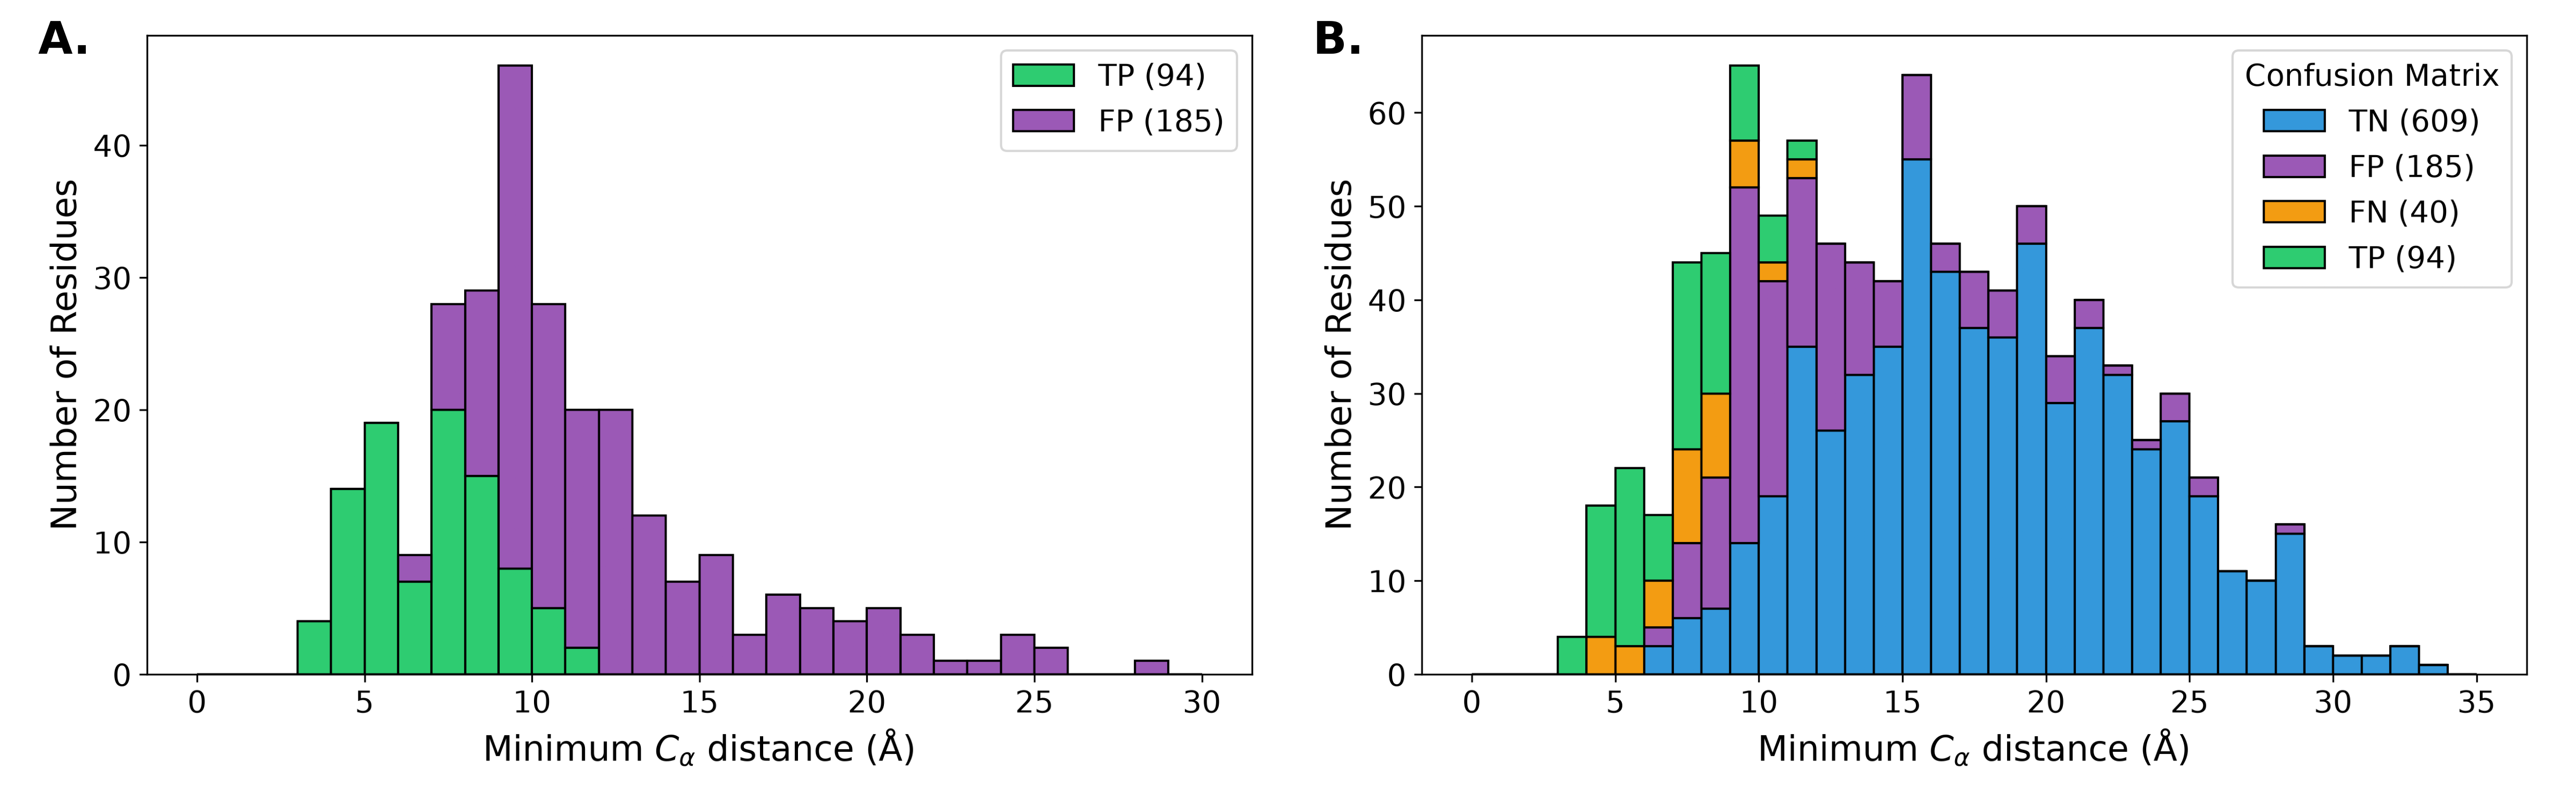
\includegraphics[width=\linewidth]{SF7_TFIIH.png}
\captionsetup{labelformat=empty}
\caption{\textbf{SI Fig. S7. Confusion Matrix Histograms for TFIIH Domain Receptors}}
\label{fig:sf7_tfiih}
\end{figure}

\clearpage
\input{../../figures/ST9_ubiquitin_domain_receptors.tex}
\clearpage

% ST10 — dissimilar apo/holo conditions (+ SF9)
% In your document preamble: \usepackage{booktabs}, \usepackage{hyperref}, \usepackage{longtable}, \usepackage{caption}
\scriptsize
\setlength{\tabcolsep}{3pt}
\begin{longtable}{llllrr@{\hspace{0.8cm}}llllrr}
\captionsetup{labelformat=empty}
\caption{\textbf{SI Table S10. Data for targets with dissimilar apo/holo experimental conditions}}
\label{tab:st10} \\
\toprule
apo\_pdb & holo\_pdb & apo\_bmrb & holo\_bmrb & F1 & MCC & apo\_pdb & holo\_pdb & apo\_bmrb & holo\_bmrb & F1 & MCC \\
\midrule
\endfirsthead
\caption[]{(continued)} \\
\toprule
apo\_pdb & holo\_pdb & apo\_bmrb & holo\_bmrb & F1 & MCC & apo\_pdb & holo\_pdb & apo\_bmrb & holo\_bmrb & F1 & MCC \\
\midrule
\endhead
\bottomrule
\endfoot
\bottomrule
\endlastfoot
 & \href{https://www.rcsb.org/structure/2MRE}{2MRE} & \href{https://bmrb.io/data_library/summary/index.php?bmrbId=25071}{25071} & \href{https://bmrb.io/data_library/summary/index.php?bmrbId=25070}{25070} & 0.80 & 0.60 &  & \href{https://www.rcsb.org/structure/6FGP}{6FGP} & \href{https://bmrb.io/data_library/summary/index.php?bmrbId=16803}{16803} & \href{https://bmrb.io/data_library/summary/index.php?bmrbId=34232}{34232} & 0.38 & 0.21 \\
 & \href{https://www.rcsb.org/structure/2MCN}{2MCN} & \href{https://bmrb.io/data_library/summary/index.php?bmrbId=16641}{16641} & \href{https://bmrb.io/data_library/summary/index.php?bmrbId=19447}{19447} & 0.68 & 0.58 &  & \href{https://www.rcsb.org/structure/7L8V}{7L8V} & \href{https://bmrb.io/data_library/summary/index.php?bmrbId=26682}{26682} & \href{https://bmrb.io/data_library/summary/index.php?bmrbId=27692}{27692} & 0.29 & 0.21 \\
 & \href{https://www.rcsb.org/structure/2N9P}{2N9P} & \href{https://bmrb.io/data_library/summary/index.php?bmrbId=25913}{25913} & \href{https://bmrb.io/data_library/summary/index.php?bmrbId=25914}{25914} & 0.72 & 0.58 &  & \href{https://www.rcsb.org/structure/2MH0}{2MH0} & \href{https://bmrb.io/data_library/summary/index.php?bmrbId=34231}{34231} & \href{https://bmrb.io/data_library/summary/index.php?bmrbId=19610}{19610} & 0.33 & 0.21 \\
 & \href{https://www.rcsb.org/structure/2AFF}{2AFF} & \href{https://bmrb.io/data_library/summary/index.php?bmrbId=5959}{5959} & \href{https://bmrb.io/data_library/summary/index.php?bmrbId=6748}{6748} & 0.62 & 0.48 &  & \href{https://www.rcsb.org/structure/2MPS}{2MPS} & \href{https://bmrb.io/data_library/summary/index.php?bmrbId=6612}{6612} & \href{https://bmrb.io/data_library/summary/index.php?bmrbId=18876}{18876} & 0.34 & 0.20 \\
 & \href{https://www.rcsb.org/structure/6IVU}{6IVU} & \href{https://bmrb.io/data_library/summary/index.php?bmrbId=36220}{36220} & \href{https://bmrb.io/data_library/summary/index.php?bmrbId=36221}{36221} & 0.67 & 0.48 &  & \href{https://www.rcsb.org/structure/2RVB}{2RVB} & \href{https://bmrb.io/data_library/summary/index.php?bmrbId=4901}{4901} & \href{https://bmrb.io/data_library/summary/index.php?bmrbId=11594}{11594} & 0.44 & 0.20 \\
\href{https://www.rcsb.org/structure/1XWH}{1XWH} & \href{https://www.rcsb.org/structure/2KE1}{2KE1} & \href{https://bmrb.io/data_library/summary/index.php?bmrbId=6374}{6374} & \href{https://bmrb.io/data_library/summary/index.php?bmrbId=16510}{16510} & 0.68 & 0.46 &  & \href{https://www.rcsb.org/structure/6U19}{6U19} & \href{https://bmrb.io/data_library/summary/index.php?bmrbId=16620}{16620} & \href{https://bmrb.io/data_library/summary/index.php?bmrbId=27875}{27875} & 0.43 & 0.20 \\
 & \href{https://www.rcsb.org/structure/6FDP}{6FDP} & \href{https://bmrb.io/data_library/summary/index.php?bmrbId=19757}{19757} & \href{https://bmrb.io/data_library/summary/index.php?bmrbId=34223}{34223} & 0.48 & 0.43 &  & \href{https://www.rcsb.org/structure/6CO4}{6CO4} & \href{https://bmrb.io/data_library/summary/index.php?bmrbId=30824}{30824} & \href{https://bmrb.io/data_library/summary/index.php?bmrbId=25979}{25979} & 0.31 & 0.20 \\
\href{https://www.rcsb.org/structure/2RQT}{2RQT} & \href{https://www.rcsb.org/structure/2RQU}{2RQU} & \href{https://bmrb.io/data_library/summary/index.php?bmrbId=11081}{11081} & \href{https://bmrb.io/data_library/summary/index.php?bmrbId=11082}{11082} & 0.60 & 0.42 &  & \href{https://www.rcsb.org/structure/2LVO}{2LVO} & \href{https://bmrb.io/data_library/summary/index.php?bmrbId=18610}{18610} & \href{https://bmrb.io/data_library/summary/index.php?bmrbId=18582}{18582} & 0.34 & 0.19 \\
\href{https://www.rcsb.org/structure/2GS0}{2GS0} & \href{https://www.rcsb.org/structure/2LOX}{2LOX} & \href{https://bmrb.io/data_library/summary/index.php?bmrbId=6225}{6225} & \href{https://bmrb.io/data_library/summary/index.php?bmrbId=18229}{18229} & 0.47 & 0.42 &  & \href{https://www.rcsb.org/structure/2LAS}{2LAS} & \href{https://bmrb.io/data_library/summary/index.php?bmrbId=50128}{50128} & \href{https://bmrb.io/data_library/summary/index.php?bmrbId=25553}{25553} & 0.28 & 0.19 \\
 & \href{https://www.rcsb.org/structure/7OVC}{7OVC} & \href{https://bmrb.io/data_library/summary/index.php?bmrbId=6546}{6546} & \href{https://bmrb.io/data_library/summary/index.php?bmrbId=34638}{34638} & 0.49 & 0.42 & \href{https://www.rcsb.org/structure/2L0I}{2L0I} & \href{https://www.rcsb.org/structure/5M9D}{5M9D} & \href{https://bmrb.io/data_library/summary/index.php?bmrbId=17044}{17044} & \href{https://bmrb.io/data_library/summary/index.php?bmrbId=34058}{34058} & 0.33 & 0.18 \\
 & \href{https://www.rcsb.org/structure/2K7A}{2K7A} & \href{https://bmrb.io/data_library/summary/index.php?bmrbId=11018}{11018} & \href{https://bmrb.io/data_library/summary/index.php?bmrbId=16809}{16809} & 0.54 & 0.42 &  & \href{https://www.rcsb.org/structure/2MMA}{2MMA} & \href{https://bmrb.io/data_library/summary/index.php?bmrbId=19849}{19849} & \href{https://bmrb.io/data_library/summary/index.php?bmrbId=19850}{19850} & 0.30 & 0.18 \\
 & \href{https://www.rcsb.org/structure/2M5A}{2M5A} & \href{https://bmrb.io/data_library/summary/index.php?bmrbId=6804}{6804} & \href{https://bmrb.io/data_library/summary/index.php?bmrbId=19043}{19043} & 0.62 & 0.42 &  & \href{https://www.rcsb.org/structure/2N83}{2N83} & \href{https://bmrb.io/data_library/summary/index.php?bmrbId=25828}{25828} & \href{https://bmrb.io/data_library/summary/index.php?bmrbId=25833}{25833} & 0.36 & 0.17 \\
\href{https://www.rcsb.org/structure/5AHT}{5AHT} & \href{https://www.rcsb.org/structure/2KPZ}{2KPZ} & \href{https://bmrb.io/data_library/summary/index.php?bmrbId=25349}{25349} & \href{https://bmrb.io/data_library/summary/index.php?bmrbId=16574}{16574} & 0.55 & 0.40 &  & \href{https://www.rcsb.org/structure/2LL7}{2LL7} & \href{https://bmrb.io/data_library/summary/index.php?bmrbId=51289}{51289} & \href{https://bmrb.io/data_library/summary/index.php?bmrbId=18028}{18028} & 0.33 & 0.17 \\
 & \href{https://www.rcsb.org/structure/2KID}{2KID} & \href{https://bmrb.io/data_library/summary/index.php?bmrbId=4879}{4879} & \href{https://bmrb.io/data_library/summary/index.php?bmrbId=16270}{16270} & 0.39 & 0.40 &  & \href{https://www.rcsb.org/structure/5IAY}{5IAY} & \href{https://bmrb.io/data_library/summary/index.php?bmrbId=30703}{30703} & \href{https://bmrb.io/data_library/summary/index.php?bmrbId=30019}{30019} & 0.22 & 0.17 \\
\href{https://www.rcsb.org/structure/2LD9}{2LD9} & \href{https://www.rcsb.org/structure/2MBH}{2MBH} & \href{https://bmrb.io/data_library/summary/index.php?bmrbId=15410}{15410} & \href{https://bmrb.io/data_library/summary/index.php?bmrbId=19399}{19399} & 0.40 & 0.40 &  & \href{https://www.rcsb.org/structure/5J7J}{5J7J} & \href{https://bmrb.io/data_library/summary/index.php?bmrbId=51289}{51289} & \href{https://bmrb.io/data_library/summary/index.php?bmrbId=30062}{30062} & 0.48 & 0.17 \\
 & \href{https://www.rcsb.org/structure/1N7T}{1N7T} & \href{https://bmrb.io/data_library/summary/index.php?bmrbId=18785}{18785} & \href{https://bmrb.io/data_library/summary/index.php?bmrbId=5631}{5631} & 0.44 & 0.40 &  & \href{https://www.rcsb.org/structure/2LXS}{2LXS} & \href{https://bmrb.io/data_library/summary/index.php?bmrbId=6095}{6095} & \href{https://bmrb.io/data_library/summary/index.php?bmrbId=18694}{18694} & 0.32 & 0.17 \\
 & \href{https://www.rcsb.org/structure/6RH6}{6RH6} & \href{https://bmrb.io/data_library/summary/index.php?bmrbId=34394}{34394} & \href{https://bmrb.io/data_library/summary/index.php?bmrbId=34395}{34395} & 0.34 & 0.38 & \href{https://www.rcsb.org/structure/2M03}{2M03} & \href{https://www.rcsb.org/structure/6IJQ}{6IJQ} & \href{https://bmrb.io/data_library/summary/index.php?bmrbId=18792}{18792} & \href{https://bmrb.io/data_library/summary/index.php?bmrbId=36133}{36133} & 0.18 & 0.16 \\
 & \href{https://www.rcsb.org/structure/2YKA}{2YKA} & \href{https://bmrb.io/data_library/summary/index.php?bmrbId=16697}{16697} & \href{https://bmrb.io/data_library/summary/index.php?bmrbId=17693}{17693} & 0.36 & 0.37 &  & \href{https://www.rcsb.org/structure/2FFK}{2FFK} & \href{https://bmrb.io/data_library/summary/index.php?bmrbId=6809}{6809} & \href{https://bmrb.io/data_library/summary/index.php?bmrbId=7024}{7024} & 0.16 & 0.15 \\
 & \href{https://www.rcsb.org/structure/2KWU}{2KWU} & \href{https://bmrb.io/data_library/summary/index.php?bmrbId=17769}{17769} & \href{https://bmrb.io/data_library/summary/index.php?bmrbId=16880}{16880} & 0.40 & 0.37 & \href{https://www.rcsb.org/structure/1N3H}{1N3H} & \href{https://www.rcsb.org/structure/2L1C}{2L1C} & \href{https://bmrb.io/data_library/summary/index.php?bmrbId=5566}{5566} & \href{https://bmrb.io/data_library/summary/index.php?bmrbId=17080}{17080} & 0.34 & 0.15 \\
\href{https://www.rcsb.org/structure/2KM4}{2KM4} & \href{https://www.rcsb.org/structure/2L0I}{2L0I} & \href{https://bmrb.io/data_library/summary/index.php?bmrbId=16411}{16411} & \href{https://bmrb.io/data_library/summary/index.php?bmrbId=17044}{17044} & 0.36 & 0.36 &  & \href{https://www.rcsb.org/structure/1LXF}{1LXF} & \href{https://bmrb.io/data_library/summary/index.php?bmrbId=30966}{30966} & \href{https://bmrb.io/data_library/summary/index.php?bmrbId=5386}{5386} & 0.37 & 0.14 \\
 & \href{https://www.rcsb.org/structure/2G3Q}{2G3Q} & \href{https://bmrb.io/data_library/summary/index.php?bmrbId=4769}{4769} & \href{https://bmrb.io/data_library/summary/index.php?bmrbId=7002}{7002} & 0.38 & 0.35 & \href{https://www.rcsb.org/structure/2JQ6}{2JQ6} & \href{https://www.rcsb.org/structure/2KFH}{2KFH} & \href{https://bmrb.io/data_library/summary/index.php?bmrbId=15279}{15279} & \href{https://bmrb.io/data_library/summary/index.php?bmrbId=16181}{16181} & 0.27 & 0.14 \\
 & \href{https://www.rcsb.org/structure/2KWV}{2KWV} & \href{https://bmrb.io/data_library/summary/index.php?bmrbId=17769}{17769} & \href{https://bmrb.io/data_library/summary/index.php?bmrbId=16885}{16885} & 0.39 & 0.34 &  & \href{https://www.rcsb.org/structure/9C5E}{9C5E} & \href{https://bmrb.io/data_library/summary/index.php?bmrbId=18610}{18610} & \href{https://bmrb.io/data_library/summary/index.php?bmrbId=31177}{31177} & 0.32 & 0.13 \\
\href{https://www.rcsb.org/structure/2LSG}{2LSG} & \href{https://www.rcsb.org/structure/2LSJ}{2LSJ} & \href{https://bmrb.io/data_library/summary/index.php?bmrbId=18431}{18431} & \href{https://bmrb.io/data_library/summary/index.php?bmrbId=18433}{18433} & 0.35 & 0.34 &  & \href{https://www.rcsb.org/structure/2KNE}{2KNE} & \href{https://bmrb.io/data_library/summary/index.php?bmrbId=51289}{51289} & \href{https://bmrb.io/data_library/summary/index.php?bmrbId=16465}{16465} & 0.36 & 0.13 \\
\href{https://www.rcsb.org/structure/2AWT}{2AWT} & \href{https://www.rcsb.org/structure/2N9E}{2N9E} & \href{https://bmrb.io/data_library/summary/index.php?bmrbId=6801}{6801} & \href{https://bmrb.io/data_library/summary/index.php?bmrbId=25901}{25901} & 0.30 & 0.33 &  & \href{https://www.rcsb.org/structure/6QXZ}{6QXZ} & \href{https://bmrb.io/data_library/summary/index.php?bmrbId=27250}{27250} & \href{https://bmrb.io/data_library/summary/index.php?bmrbId=27251}{27251} & 0.42 & 0.13 \\
 & \href{https://www.rcsb.org/structure/2JXC}{2JXC} & \href{https://bmrb.io/data_library/summary/index.php?bmrbId=4184}{4184} & \href{https://bmrb.io/data_library/summary/index.php?bmrbId=15554}{15554} & 0.58 & 0.33 &  & \href{https://www.rcsb.org/structure/1ONV}{1ONV} & \href{https://bmrb.io/data_library/summary/index.php?bmrbId=27288}{27288} & \href{https://bmrb.io/data_library/summary/index.php?bmrbId=5685}{5685} & 0.34 & 0.12 \\
\href{https://www.rcsb.org/structure/2GS0}{2GS0} & \href{https://www.rcsb.org/structure/2MKR}{2MKR} & \href{https://bmrb.io/data_library/summary/index.php?bmrbId=6225}{6225} & \href{https://bmrb.io/data_library/summary/index.php?bmrbId=19791}{19791} & 0.29 & 0.33 & \href{https://www.rcsb.org/structure/2KJD}{2KJD} & \href{https://www.rcsb.org/structure/2M0V}{2M0V} & \href{https://bmrb.io/data_library/summary/index.php?bmrbId=16637}{16637} & \href{https://bmrb.io/data_library/summary/index.php?bmrbId=18826}{18826} & 0.20 & 0.11 \\
\href{https://www.rcsb.org/structure/2GS0}{2GS0} & \href{https://www.rcsb.org/structure/2N0Y}{2N0Y} & \href{https://bmrb.io/data_library/summary/index.php?bmrbId=6225}{6225} & \href{https://bmrb.io/data_library/summary/index.php?bmrbId=25540}{25540} & 0.37 & 0.33 & \href{https://www.rcsb.org/structure/1V49}{1V49} & \href{https://www.rcsb.org/structure/2LUE}{2LUE} & \href{https://bmrb.io/data_library/summary/index.php?bmrbId=5958}{5958} & \href{https://bmrb.io/data_library/summary/index.php?bmrbId=18518}{18518} & 0.22 & 0.11 \\
 & \href{https://www.rcsb.org/structure/2KSP}{2KSP} & \href{https://bmrb.io/data_library/summary/index.php?bmrbId=15279}{15279} & \href{https://bmrb.io/data_library/summary/index.php?bmrbId=16671}{16671} & 0.40 & 0.32 &  & \href{https://www.rcsb.org/structure/2M86}{2M86} & \href{https://bmrb.io/data_library/summary/index.php?bmrbId=15945}{15945} & \href{https://bmrb.io/data_library/summary/index.php?bmrbId=19230}{19230} & 0.25 & 0.10 \\
\href{https://www.rcsb.org/structure/2LPC}{2LPC} & \href{https://www.rcsb.org/structure/2M04}{2M04} & \href{https://bmrb.io/data_library/summary/index.php?bmrbId=18250}{18250} & \href{https://bmrb.io/data_library/summary/index.php?bmrbId=18793}{18793} & 0.45 & 0.31 &  & \href{https://www.rcsb.org/structure/2MCN}{2MCN} & \href{https://bmrb.io/data_library/summary/index.php?bmrbId=18610}{18610} & \href{https://bmrb.io/data_library/summary/index.php?bmrbId=19447}{19447} & 0.40 & 0.10 \\
 & \href{https://www.rcsb.org/structure/2BN5}{2BN5} & \href{https://bmrb.io/data_library/summary/index.php?bmrbId=6691}{6691} & \href{https://bmrb.io/data_library/summary/index.php?bmrbId=6690}{6690} & 0.28 & 0.31 &  & \href{https://www.rcsb.org/structure/2N1A}{2N1A} & \href{https://bmrb.io/data_library/summary/index.php?bmrbId=6304}{6304} & \href{https://bmrb.io/data_library/summary/index.php?bmrbId=25553}{25553} & 0.10 & 0.10 \\
 & \href{https://www.rcsb.org/structure/2KGI}{2KGI} & \href{https://bmrb.io/data_library/summary/index.php?bmrbId=16209}{16209} & \href{https://bmrb.io/data_library/summary/index.php?bmrbId=16210}{16210} & 0.62 & 0.30 &  & \href{https://www.rcsb.org/structure/5XV8}{5XV8} & \href{https://bmrb.io/data_library/summary/index.php?bmrbId=4901}{4901} & \href{https://bmrb.io/data_library/summary/index.php?bmrbId=36101}{36101} & 0.37 & 0.09 \\
\href{https://www.rcsb.org/structure/5AHT}{5AHT} & \href{https://www.rcsb.org/structure/2KQ0}{2KQ0} & \href{https://bmrb.io/data_library/summary/index.php?bmrbId=25349}{25349} & \href{https://bmrb.io/data_library/summary/index.php?bmrbId=16575}{16575} & 0.50 & 0.30 &  & \href{https://www.rcsb.org/structure/2KA6}{2KA6} & \href{https://bmrb.io/data_library/summary/index.php?bmrbId=4789}{4789} & \href{https://bmrb.io/data_library/summary/index.php?bmrbId=16015}{16015} & 0.51 & 0.09 \\
 & \href{https://www.rcsb.org/structure/2RUK}{2RUK} & \href{https://bmrb.io/data_library/summary/index.php?bmrbId=4901}{4901} & \href{https://bmrb.io/data_library/summary/index.php?bmrbId=11578}{11578} & 0.44 & 0.30 &  & \href{https://www.rcsb.org/structure/6XMN}{6XMN} & \href{https://bmrb.io/data_library/summary/index.php?bmrbId=30316}{30316} & \href{https://bmrb.io/data_library/summary/index.php?bmrbId=50331}{50331} & 0.40 & 0.09 \\
 & \href{https://www.rcsb.org/structure/2RQG}{2RQG} & \href{https://bmrb.io/data_library/summary/index.php?bmrbId=4915}{4915} & \href{https://bmrb.io/data_library/summary/index.php?bmrbId=10019}{10019} & 0.43 & 0.30 &  & \href{https://www.rcsb.org/structure/2MGU}{2MGU} & \href{https://bmrb.io/data_library/summary/index.php?bmrbId=51289}{51289} & \href{https://bmrb.io/data_library/summary/index.php?bmrbId=19604}{19604} & 0.42 & 0.09 \\
 & \href{https://www.rcsb.org/structure/2MS4}{2MS4} & \href{https://bmrb.io/data_library/summary/index.php?bmrbId=2208}{2208} & \href{https://bmrb.io/data_library/summary/index.php?bmrbId=25104}{25104} & 0.29 & 0.29 &  & \href{https://www.rcsb.org/structure/2KJE}{2KJE} & \href{https://bmrb.io/data_library/summary/index.php?bmrbId=4789}{4789} & \href{https://bmrb.io/data_library/summary/index.php?bmrbId=16318}{16318} & 0.45 & 0.07 \\
 & \href{https://www.rcsb.org/structure/2KPL}{2KPL} & \href{https://bmrb.io/data_library/summary/index.php?bmrbId=6911}{6911} & \href{https://bmrb.io/data_library/summary/index.php?bmrbId=16559}{16559} & 0.40 & 0.28 &  & \href{https://www.rcsb.org/structure/2L53}{2L53} & \href{https://bmrb.io/data_library/summary/index.php?bmrbId=51289}{51289} & \href{https://bmrb.io/data_library/summary/index.php?bmrbId=17264}{17264} & 0.27 & 0.06 \\
 & \href{https://www.rcsb.org/structure/2MPM}{2MPM} & \href{https://bmrb.io/data_library/summary/index.php?bmrbId=4155}{4155} & \href{https://bmrb.io/data_library/summary/index.php?bmrbId=19989}{19989} & 0.41 & 0.28 &  & \href{https://www.rcsb.org/structure/2MZD}{2MZD} & \href{https://bmrb.io/data_library/summary/index.php?bmrbId=34231}{34231} & \href{https://bmrb.io/data_library/summary/index.php?bmrbId=25484}{25484} & 0.35 & 0.06 \\
 & \href{https://www.rcsb.org/structure/2MG5}{2MG5} & \href{https://bmrb.io/data_library/summary/index.php?bmrbId=51289}{51289} & \href{https://bmrb.io/data_library/summary/index.php?bmrbId=19586}{19586} & 0.44 & 0.27 &  & \href{https://www.rcsb.org/structure/6BUT}{6BUT} & \href{https://bmrb.io/data_library/summary/index.php?bmrbId=51289}{51289} & \href{https://bmrb.io/data_library/summary/index.php?bmrbId=27095}{27095} & 0.25 & 0.04 \\
 & \href{https://www.rcsb.org/structure/5JYV}{5JYV} & \href{https://bmrb.io/data_library/summary/index.php?bmrbId=30091}{30091} & \href{https://bmrb.io/data_library/summary/index.php?bmrbId=30093}{30093} & 0.45 & 0.27 &  & \href{https://www.rcsb.org/structure/2MZP}{2MZP} & \href{https://bmrb.io/data_library/summary/index.php?bmrbId=30966}{30966} & \href{https://bmrb.io/data_library/summary/index.php?bmrbId=25495}{25495} & 0.17 & 0.04 \\
 & \href{https://www.rcsb.org/structure/2M0G}{2M0G} & \href{https://bmrb.io/data_library/summary/index.php?bmrbId=19034}{19034} & \href{https://bmrb.io/data_library/summary/index.php?bmrbId=18808}{18808} & 0.43 & 0.27 &  & \href{https://www.rcsb.org/structure/9R3Y}{9R3Y} & \href{https://bmrb.io/data_library/summary/index.php?bmrbId=26643}{26643} & \href{https://bmrb.io/data_library/summary/index.php?bmrbId=34992}{34992} & 0.25 & 0.04 \\
\href{https://www.rcsb.org/structure/5YDY}{5YDY} & \href{https://www.rcsb.org/structure/2LAW}{2LAW} & \href{https://bmrb.io/data_library/summary/index.php?bmrbId=36115}{36115} & \href{https://bmrb.io/data_library/summary/index.php?bmrbId=17538}{17538} & 0.50 & 0.27 &  & \href{https://www.rcsb.org/structure/2MKP}{2MKP} & \href{https://bmrb.io/data_library/summary/index.php?bmrbId=25495}{25495} & \href{https://bmrb.io/data_library/summary/index.php?bmrbId=19789}{19789} & 0.27 & 0.04 \\
 & \href{https://www.rcsb.org/structure/1CF4}{1CF4} & \href{https://bmrb.io/data_library/summary/index.php?bmrbId=18251}{18251} & \href{https://bmrb.io/data_library/summary/index.php?bmrbId=4700}{4700} & 0.49 & 0.27 &  & \href{https://www.rcsb.org/structure/2LZ6}{2LZ6} & \href{https://bmrb.io/data_library/summary/index.php?bmrbId=15407}{15407} & \href{https://bmrb.io/data_library/summary/index.php?bmrbId=18737}{18737} & 0.28 & 0.02 \\
 & \href{https://www.rcsb.org/structure/2N3K}{2N3K} & \href{https://bmrb.io/data_library/summary/index.php?bmrbId=15125}{15125} & \href{https://bmrb.io/data_library/summary/index.php?bmrbId=25649}{25649} & 0.39 & 0.26 &  & \href{https://www.rcsb.org/structure/7NQC}{7NQC} & \href{https://bmrb.io/data_library/summary/index.php?bmrbId=51289}{51289} & \href{https://bmrb.io/data_library/summary/index.php?bmrbId=34608}{34608} & 0.34 & 0.01 \\
 & \href{https://www.rcsb.org/structure/2M0G}{2M0G} & \href{https://bmrb.io/data_library/summary/index.php?bmrbId=18802}{18802} & \href{https://bmrb.io/data_library/summary/index.php?bmrbId=18808}{18808} & 0.29 & 0.25 &  & \href{https://www.rcsb.org/structure/7F7X}{7F7X} & \href{https://bmrb.io/data_library/summary/index.php?bmrbId=17769}{17769} & \href{https://bmrb.io/data_library/summary/index.php?bmrbId=36427}{36427} & 0.20 & 0.00 \\
 & \href{https://www.rcsb.org/structure/2MOW}{2MOW} & \href{https://bmrb.io/data_library/summary/index.php?bmrbId=17173}{17173} & \href{https://bmrb.io/data_library/summary/index.php?bmrbId=19954}{19954} & 0.21 & 0.25 &  & \href{https://www.rcsb.org/structure/6B1G}{6B1G} & \href{https://bmrb.io/data_library/summary/index.php?bmrbId=27072}{27072} & \href{https://bmrb.io/data_library/summary/index.php?bmrbId=30345}{30345} & 0.26 & -0.01 \\
 & \href{https://www.rcsb.org/structure/2MBB}{2MBB} & \href{https://bmrb.io/data_library/summary/index.php?bmrbId=15410}{15410} & \href{https://bmrb.io/data_library/summary/index.php?bmrbId=19394}{19394} & 0.43 & 0.24 & \href{https://www.rcsb.org/structure/2E5E}{2E5E} & \href{https://www.rcsb.org/structure/2L7U}{2L7U} & \href{https://bmrb.io/data_library/summary/index.php?bmrbId=7364}{7364} & \href{https://bmrb.io/data_library/summary/index.php?bmrbId=17378}{17378} & 0.14 & -0.01 \\
 & \href{https://www.rcsb.org/structure/2KNH}{2KNH} & \href{https://bmrb.io/data_library/summary/index.php?bmrbId=7396}{7396} & \href{https://bmrb.io/data_library/summary/index.php?bmrbId=16467}{16467} & 0.30 & 0.24 & \href{https://www.rcsb.org/structure/5YDX}{5YDX} & \href{https://www.rcsb.org/structure/2LAY}{2LAY} & \href{https://bmrb.io/data_library/summary/index.php?bmrbId=36114}{36114} & \href{https://bmrb.io/data_library/summary/index.php?bmrbId=17540}{17540} & 0.29 & -0.01 \\
 & \href{https://www.rcsb.org/structure/2N3A}{2N3A} & \href{https://bmrb.io/data_library/summary/index.php?bmrbId=34537}{34537} & \href{https://bmrb.io/data_library/summary/index.php?bmrbId=25639}{25639} & 0.37 & 0.24 &  & \href{https://www.rcsb.org/structure/2JMX}{2JMX} & \href{https://bmrb.io/data_library/summary/index.php?bmrbId=6564}{6564} & \href{https://bmrb.io/data_library/summary/index.php?bmrbId=15072}{15072} & 0.09 & -0.01 \\
\href{https://www.rcsb.org/structure/2L0I}{2L0I} & \href{https://www.rcsb.org/structure/5LVF}{5LVF} & \href{https://bmrb.io/data_library/summary/index.php?bmrbId=17044}{17044} & \href{https://bmrb.io/data_library/summary/index.php?bmrbId=34041}{34041} & 0.31 & 0.24 &  & \href{https://www.rcsb.org/structure/2N8J}{2N8J} & \href{https://bmrb.io/data_library/summary/index.php?bmrbId=51289}{51289} & \href{https://bmrb.io/data_library/summary/index.php?bmrbId=25852}{25852} & 0.19 & -0.01 \\
\href{https://www.rcsb.org/structure/2GS0}{2GS0} & \href{https://www.rcsb.org/structure/2M14}{2M14} & \href{https://bmrb.io/data_library/summary/index.php?bmrbId=6225}{6225} & \href{https://bmrb.io/data_library/summary/index.php?bmrbId=18842}{18842} & 0.24 & 0.23 &  & \href{https://www.rcsb.org/structure/2M55}{2M55} & \href{https://bmrb.io/data_library/summary/index.php?bmrbId=51289}{51289} & \href{https://bmrb.io/data_library/summary/index.php?bmrbId=19036}{19036} & 0.24 & -0.01 \\
 & \href{https://www.rcsb.org/structure/1I5H}{1I5H} & \href{https://bmrb.io/data_library/summary/index.php?bmrbId=26698}{26698} & \href{https://bmrb.io/data_library/summary/index.php?bmrbId=4963}{4963} & 0.40 & 0.23 &  & \href{https://www.rcsb.org/structure/2RMK}{2RMK} & \href{https://bmrb.io/data_library/summary/index.php?bmrbId=5511}{5511} & \href{https://bmrb.io/data_library/summary/index.php?bmrbId=11010}{11010} & 0.18 & -0.02 \\
 & \href{https://www.rcsb.org/structure/2IPA}{2IPA} & \href{https://bmrb.io/data_library/summary/index.php?bmrbId=6075}{6075} & \href{https://bmrb.io/data_library/summary/index.php?bmrbId=15028}{15028} & 0.18 & 0.23 &  & \href{https://www.rcsb.org/structure/2NBV}{2NBV} & \href{https://bmrb.io/data_library/summary/index.php?bmrbId=30824}{30824} & \href{https://bmrb.io/data_library/summary/index.php?bmrbId=25995}{25995} & 0.15 & -0.02 \\
 & \href{https://www.rcsb.org/structure/2KWI}{2KWI} & \href{https://bmrb.io/data_library/summary/index.php?bmrbId=15230}{15230} & \href{https://bmrb.io/data_library/summary/index.php?bmrbId=15525}{15525} & 0.36 & 0.23 &  & \href{https://www.rcsb.org/structure/5TP6}{5TP6} & \href{https://bmrb.io/data_library/summary/index.php?bmrbId=51289}{51289} & \href{https://bmrb.io/data_library/summary/index.php?bmrbId=30196}{30196} & 0.21 & -0.03 \\
 & \href{https://www.rcsb.org/structure/2MZW}{2MZW} & \href{https://bmrb.io/data_library/summary/index.php?bmrbId=25368}{25368} & \href{https://bmrb.io/data_library/summary/index.php?bmrbId=25504}{25504} & 0.29 & 0.23 &  & \href{https://www.rcsb.org/structure/2MNU}{2MNU} & \href{https://bmrb.io/data_library/summary/index.php?bmrbId=4283}{4283} & \href{https://bmrb.io/data_library/summary/index.php?bmrbId=19906}{19906} & 0.19 & -0.04 \\
\href{https://www.rcsb.org/structure/2GS0}{2GS0} & \href{https://www.rcsb.org/structure/5URN}{5URN} & \href{https://bmrb.io/data_library/summary/index.php?bmrbId=6225}{6225} & \href{https://bmrb.io/data_library/summary/index.php?bmrbId=30243}{30243} & 0.29 & 0.23 &  & \href{https://www.rcsb.org/structure/2LV6}{2LV6} & \href{https://bmrb.io/data_library/summary/index.php?bmrbId=51289}{51289} & \href{https://bmrb.io/data_library/summary/index.php?bmrbId=18556}{18556} & 0.35 & -0.07 \\
\href{https://www.rcsb.org/structure/1U2N}{1U2N} & \href{https://www.rcsb.org/structure/1L8C}{1L8C} & \href{https://bmrb.io/data_library/summary/index.php?bmrbId=6268}{6268} & \href{https://bmrb.io/data_library/summary/index.php?bmrbId=5327}{5327} & 0.58 & 0.22 &  & \href{https://www.rcsb.org/structure/2L29}{2L29} & \href{https://bmrb.io/data_library/summary/index.php?bmrbId=34000}{34000} & \href{https://bmrb.io/data_library/summary/index.php?bmrbId=17127}{17127} & 0.16 & -0.08 \\
\href{https://www.rcsb.org/structure/2GS0}{2GS0} & \href{https://www.rcsb.org/structure/2N23}{2N23} & \href{https://bmrb.io/data_library/summary/index.php?bmrbId=6225}{6225} & \href{https://bmrb.io/data_library/summary/index.php?bmrbId=25584}{25584} & 0.17 & 0.22 &  & \href{https://www.rcsb.org/structure/9C5E}{9C5E} & \href{https://bmrb.io/data_library/summary/index.php?bmrbId=18642}{18642} & \href{https://bmrb.io/data_library/summary/index.php?bmrbId=31177}{31177} & 0.35 & -0.11 \\
 & \href{https://www.rcsb.org/structure/6OQJ}{6OQJ} & \href{https://bmrb.io/data_library/summary/index.php?bmrbId=4276}{4276} & \href{https://bmrb.io/data_library/summary/index.php?bmrbId=30605}{30605} & 0.32 & 0.22 &  & \href{https://www.rcsb.org/structure/2N80}{2N80} & \href{https://bmrb.io/data_library/summary/index.php?bmrbId=51835}{51835} & \href{https://bmrb.io/data_library/summary/index.php?bmrbId=25829}{25829} & 0.04 & -0.13 \\
 & \href{https://www.rcsb.org/structure/2LL6}{2LL6} & \href{https://bmrb.io/data_library/summary/index.php?bmrbId=51289}{51289} & \href{https://bmrb.io/data_library/summary/index.php?bmrbId=18027}{18027} & 0.39 & 0.21 &  & \href{https://www.rcsb.org/structure/2RSE}{2RSE} & \href{https://bmrb.io/data_library/summary/index.php?bmrbId=16931}{16931} & \href{https://bmrb.io/data_library/summary/index.php?bmrbId=11471}{11471} & 0.00 & -0.16 \\
\href{https://www.rcsb.org/structure/1U2N}{1U2N} & \href{https://www.rcsb.org/structure/2KA4}{2KA4} & \href{https://bmrb.io/data_library/summary/index.php?bmrbId=6268}{6268} & \href{https://bmrb.io/data_library/summary/index.php?bmrbId=16014}{16014} & 0.55 & 0.21 &  & \href{https://www.rcsb.org/structure/2RS9}{2RS9} & \href{https://bmrb.io/data_library/summary/index.php?bmrbId=19125}{19125} & \href{https://bmrb.io/data_library/summary/index.php?bmrbId=11463}{11463} & 0.00 & -0.17 \\
\end{longtable}

\begin{figure}[htbp]
\centering
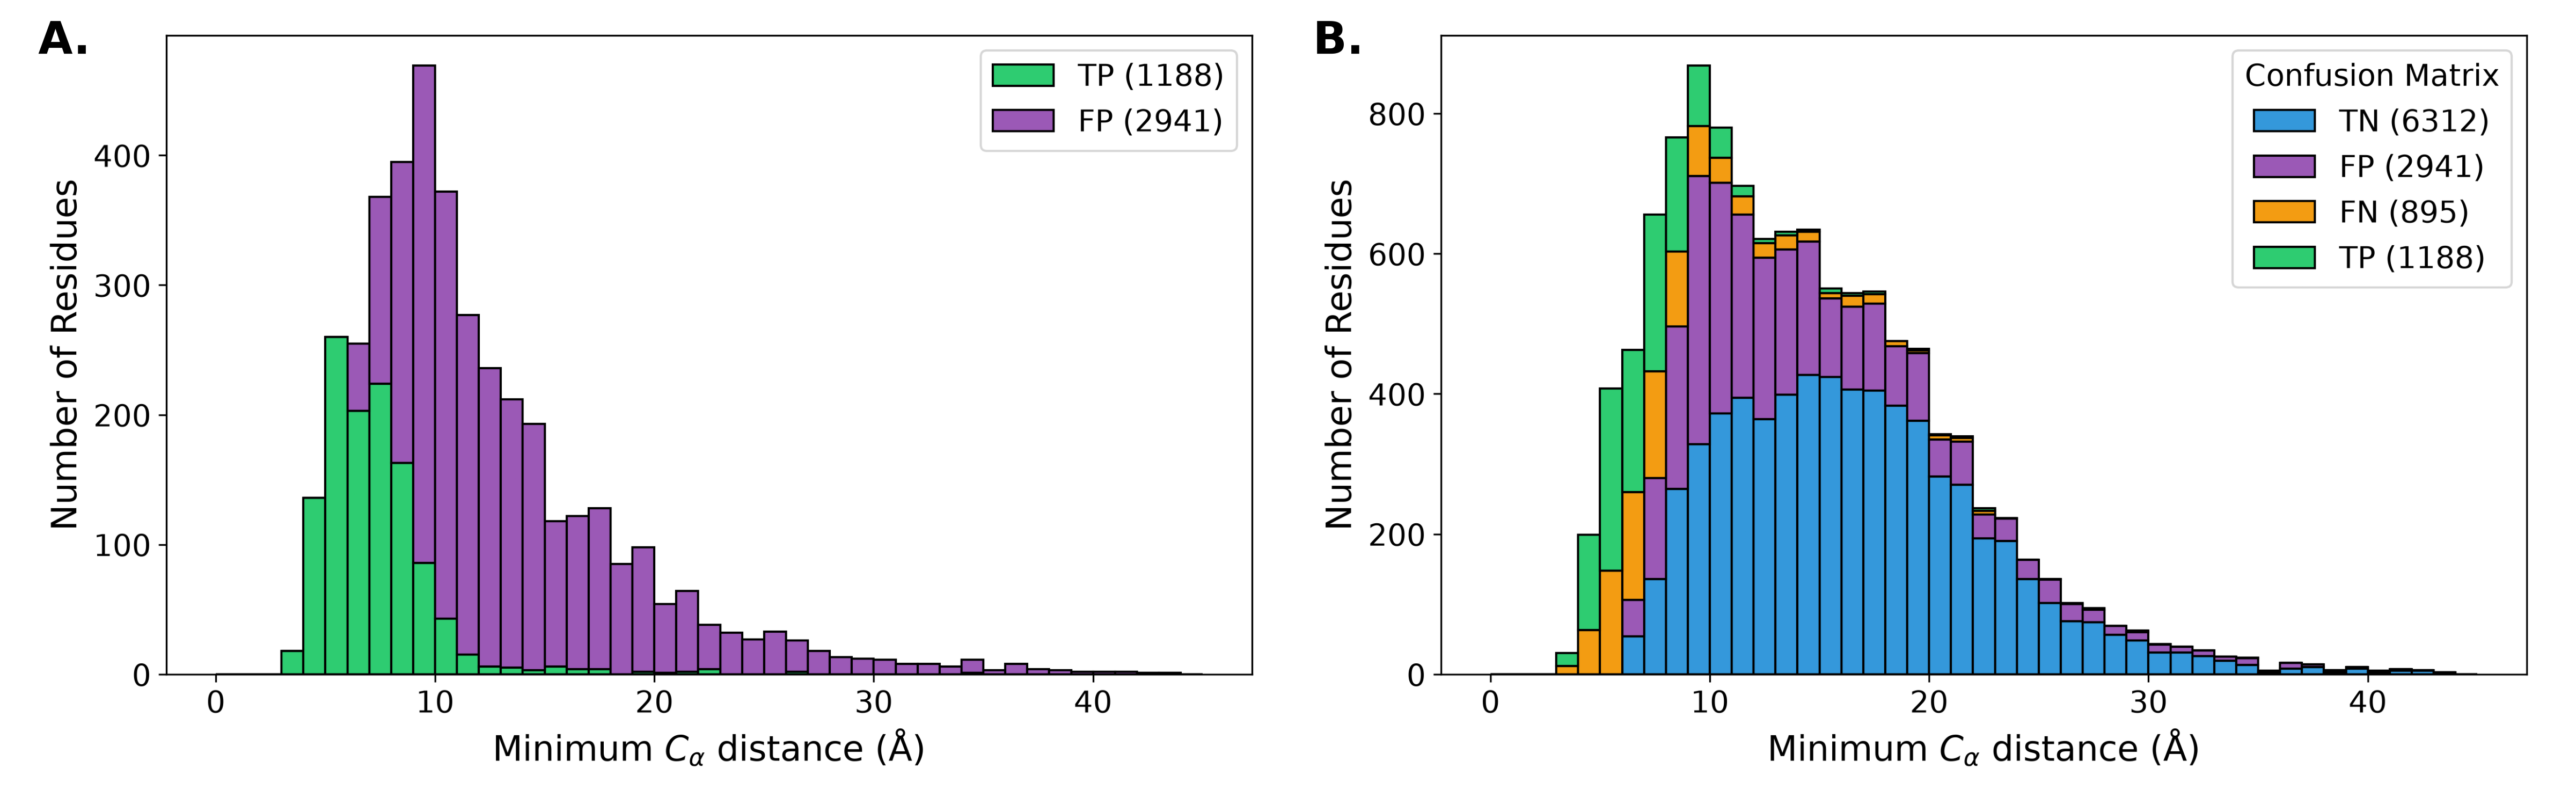
\includegraphics[width=\linewidth]{SF9_dissimilar_apo_holo_conditions.png}
\captionsetup{labelformat=empty}
\caption{\textbf{SI Fig. S9. Confusion Matrix Histograms for targets with dissimilar apo/holo experimental conditions}}
\label{fig:sf9_dissimilar_apo_holo_conditions}
\end{figure}


\end{document}
